%%
%% This is file `sample-sigplan.tex',
%% generated with the docstrip utility.
%%
%% The original source files were:
%%
%% samples.dtx  (with options: `sigplan')
%% 
%% IMPORTANT NOTICE:
%% 
%% For the copyright see the source file.
%% 
%% Any modified versions of this file must be renamed
%% with new filenames distinct from sample-sigplan.tex.
%% 
%% For distribution of the original source see the terms
%% for copying and modification in the file samples.dtx.
%% 
%% This generated file may be distributed as long as the
%% original source files, as listed above, are part of the
%% same distribution. (The sources need not necessarily be
%% in the same archive or directory.)
%%
%% The first command in your LaTeX source must be the \documentclass command.
\documentclass[sigplan,screen]{acmart}

%%
%% \BibTeX command to typeset BibTeX logo in the docs
\AtBeginDocument{%
  \providecommand\BibTeX{{%
    \normalfont B\kern-0.5em{\scshape i\kern-0.25em b}\kern-0.8em\TeX}}}

%%% The following is specific to PEPM '21 and the paper
%%% 'Efficient Fair Conjunction for Structurally-Recursive Relations'
%%% by Peter Lozov and Dmitry Boulytchev.
%%%
\setcopyright{acmcopyright}
\acmPrice{15.00}
\acmDOI{10.1145/3441296.3441397}
\acmYear{2021}
\copyrightyear{2021}
\acmSubmissionID{poplws21pepmmain-p20-p}
\acmISBN{978-1-4503-8305-9/21/01}
\acmConference[PEPM '21]{Proceedings of the 2021 ACM SIGPLAN Workshop on Partial Evaluation and Program Manipulation}{January 18--19, 2021}{Virtual, Denmark}
\acmBooktitle{Proceedings of the 2021 ACM SIGPLAN Workshop on Partial Evaluation and Program Manipulation (PEPM '21), January 18--19, 2021, Virtual, Denmark}


% \usepackage[T2A]{fontenc}
\usepackage[utf8]{inputenc}

\usepackage[english]{babel}
\usepackage{listings}
\usepackage[section]{placeins}
\usepackage{multirow}
\usepackage{pgfplots}
\usepackage{yfonts}
\usepackage{subcaption}
\usepackage{xspace}
% \usepackage{amssymb}
\usepackage{amsmath}
\usepackage{comment}
\usepackage{url}
\usepackage{tikz}
\usetikzlibrary{trees}

%\pgfplotsset{width=7cm,compat=1.8}

\lstdefinelanguage{ocanren}{
keywords={run, conde, fresh, let, in, match, with, when, class, type,
object, method, of, rec, until, while, not, do, done, as, val, inherit,
new, module, sig, deriving, datatype, struct, if, then, else, open, private, virtual, include, success, failure,
true, false},
sensitive=true,
commentstyle=\small\itshape\ttfamily,
keywordstyle=\textbf,%\ttfamily\underline,
identifierstyle=\ttfamily,
basewidth={0.5em,0.5em},
columns=fixed,
mathescape=true,
fontadjust=true,
literate={fun}{{$\lambda$}}1 {->}{{$\to$}}3 {===}{{$\equiv$}}1 {=/=}{{$\not\equiv$}}1 {|>}{{$\triangleright$}}3 {\\/}{{$\vee$}}2 {/\\}{{$\wedge$}}2 {^}{{$\uparrow$}}1,
morecomment=[s]{(*}{*)} %,
%numbers=left
}

\lstset{
language=ocanren
}

\newcommand{\ruleno}[1]{\mbox{[\textsc{#1}]}}
\newcommand{\rulen}[1]{[\textsc{#1}]}
\newcommand{\mk}{\textsc{miniKanren}\xspace}
\newcommand{\inbr}[1]{\langle #1 \rangle}
\renewcommand{\emptyset}{\varnothing}
\newcommand{\primi}[1]{\mbox{\bf #1}}

\newenvironment{proofsketch}{%
  \renewcommand{\proofname}{Proof sketch}\proof}{\endproof}

\makeatletter
\newcommand{\xdashrightarrow}[2][]{\ext@arrow 0359\rightarrowfill@@{#1}{#2}}
\def\rightarrowfill@@{\arrowfill@@\relax\relbar\rightarrow}
\def\arrowfill@@#1#2#3#4{%
  $\m@th\thickmuskip0mu\medmuskip\thickmuskip\thinmuskip\thickmuskip
   \relax#4#1
   \xleaders\hbox{$#4#2$}\hfill
   #3$%
}
\makeatother

%%
%% Submission ID.
%% Use this when submitting an article to a sponsored event. You'll
%% receive a unique submission ID from the organizers
%% of the event, and this ID should be used as the parameter to this command.
%%\acmSubmissionID{123-A56-BU3}

%%
%% The majority of ACM publications use numbered citations and
%% references.  The command \citestyle{authoryear} switches to the
%% "author year" style.
%%
%% If you are preparing content for an event
%% sponsored by ACM SIGGRAPH, you must use the "author year" style of
%% citations and references.
%% Uncommenting
%% the next command will enable that style.
%%\citestyle{acmauthoryear}

%%
%% end of the preamble, start of the body of the document source.
\sloppy
\begin{document}

%%
%% The "title" command has an optional parameter,
%% allowing the author to define a "short title" to be used in page headers.
\title[Efficient Fair Conjunction for Structurally-Recursive Relations]
      {Efficient Fair Conjunction for\\ Structurally-Recursive Relations}
\titlenote{The reported study was funded by RFBR, projects number 18-01-00380 and 19-31-90053.}

%%
%% The "author" command and its associated commands are used to define
%% the authors and their affiliations.
%% Of note is the shared affiliation of the first two authors, and the
%% "authornote" and "authornotemark" commands
%% used to denote shared contribution to the research.
\author{Peter Lozov}
%\authornote{Both authors contributed equally to this research.}
\email{lozov.peter@gmail.com}
\orcid{0000-0003-3563-2828}
\author{Dmitry Boulytchev}
%\authornotemark[1]
\email{dboulytchev@math.spbu.ru}
\orcid{0000-0001-8363-7143}
\affiliation{%
  \institution{St.Petersburg State University, JetBrains Research}
  \streetaddress{P.O. Box 1212}
  \city{St.Petersburg}
  \country{Russia}
  \postcode{43017-6221}
}
%%
%% By default, the full list of authors will be used in the page
%% headers. Often, this list is too long, and will overlap
%% other information printed in the page headers. This command allows
%% the author to define a more concise list
%% of authors' names for this purpose.
% \renewcommand{\shortauthors}{Lozov and Boulytchev}

%%
%% The abstract is a short summary of the work to be presented in the
%% article.
\begin{abstract}
  We present a new, \emph{fair}, conjunction evaluation strategy for relational programming language \mk. Unlike the original left-biased
  conjunction, our approach controls the order of conjunct execution based on the intrinsic properties of relation definitions.
  We present both the formal study of conjunction fairness and practical evaluation, which demonstrates the essential
  improvement in terms of both performance and convergence.
\end{abstract}

%%
%% The code below is generated by the tool at http://dl.acm.org/ccs.cfm.
%% Please copy and paste the code instead of the example below.
%%
\begin{CCSXML}
<ccs2012>
<concept>
<concept_id>10003752.10010124.10010131.10010134</concept_id>
<concept_desc>Theory of computation~Operational semantics</concept_desc>
<concept_significance>500</concept_significance>
</concept>
<concept>
<concept_id>10003752.10003790.10003795</concept_id>
<concept_desc>Theory of computation~Constraint and logic programming</concept_desc>
<concept_significance>500</concept_significance>
</concept>
</ccs2012>
\end{CCSXML}

\ccsdesc[500]{Theory of computation~Operational semantics}
\ccsdesc[500]{Theory of computation~Constraint and logic programming}

%%
%% Keywords. The author(s) should pick words that accurately describe
%% the work being presented. Separate the keywords with commas.
\keywords{relational programming, miniKanren, evaluation strategies, operational semantics}

%% A "teaser" image appears between the author and affiliation
%% information and the body of the document, and typically spans the
%% page.
%\begin{teaserfigure}
%  \includegraphics[width=\textwidth]{sampleteaser}
%  \caption{Seattle Mariners at Spring Training, 2010.}
%  \Description{Enjoying the baseball game from the third-base
%  seats. Ichiro Suzuki preparing to bat.}
%  \label{fig:teaser}
%\end{teaserfigure}

%%
%% This command processes the author and affiliation and title
%% information and builds the first part of the formatted document.
\maketitle

\begin{comment}
  
  Reviewer 1:
  
  2. The case studies that the evaluation section is based on seem somewhat small and toyish. Please say something about how representative they are.
  
  4. S3: You describe => as a "big-step" arrow, but it looks small-step to me?

  Fig. 2: Please clarify whether this small-step semantics is from [20] or somewhere else?

  I would have liked to have seen more summary information in the table in Figure 9 to show to ratio in timings between the three different semantics.

  Does the “naive semantics” correspond to a form of iterative deepening?
\end{comment}

\section{Introduction}

Relational programming is an approach, based on the idea of describing programs not as functions, but 
as relations, without distinguishing between the arguments and the result value. This technique makes it 
possible to ``query'' programs in various ways, for example, to execute them ``backwards'', finding
all sets of arguments for a given result. Relational behavior can be reproduced using a number of
logic programming languages, such as Prolog, Mercury~\cite{Mercury}, 
or Curry~\cite{Curry}. 
There is also a family of embedded DSLs, specifically designed for writing declarative relational
programs that originates from \miniKanren~\cite{TRS}. \miniKanren is a minimalistic 
declarative language, initially developed for Scheme/Racket. The smallest implementation of \miniKanren 
is reported to comprise of only 40 LOC~\cite{MicroKanren,2016}; there are also more elaborate versions, including
\miniKanren with constraints~\cite{CKanren,CKanren1}, user-assisted search~\cite{Guided}, nominal unification~\cite{AlphaKanren},
etc. Due to its simplicity, \miniKanren was implemented for more than 50 other languages, such as
Haskell, Go, Smalltalk, and OCaml. In a nutshell, miniKanren introduces a minimalistic set of constructs to describe
relations over a set of syntactic terms, thus providing the same expressivity as a pure core of conventional
logic programming\footnote{A detailed miniKanren to Prolog comparison can be found at \url{http://minikanren.org/minikanren-and-prolog.html}}. 

\miniKanren has proven to be a useful tool to provide elegant solutions for various problems, otherwise considered as
non-trivial~\cite{WillThesis}. One of the most promising areas of application for \miniKanren is the implementation of
\emph{relational interpreters}. Such interpreters are capable not only to interpret programs in various directions, but also
to infer programs on the basis of expected input-output specification~\cite{Untagged}.

Being quite simple and easy to use by design, in implementation \miniKanren introduces some subtleties. Under the hood, \miniKanren 
uses a complete interleaving search~\cite{Search}. This search is guaranteed to find all existing solutions; however, it can diverge, when no 
solution exists. In reality, this amounts to divergence in a number of important cases~--- for example, when a program is asked to 
return \emph{all} existing solutions, or when the number of requested solutions exceeds the number of existing ones.
It is often possible to refactor the specification of a concrete query to avoid the divergence, but this has to be done for every execution
``direction'' of interest that compromises the idea of fully declarative relational programming.

The specifications that do not diverge even when no solutions exist, are called \emph{refutationally complete}~\cite{WillThesis}. Writing 
refutationally complete relational specifications nowadays requires knowledge of \miniKanren implementation intrinsics, and is not always
possible due to the undecidability of the fundamental computability problems. However, by developing a more advanced search it is possible
to make more specifications refutationally complete.

In this work we address one particular problem that often leads to refutational incompleteness~--- the non-commutativity of
conjunction. We present an optimization technique that is based on a certain non-termination test. Our optimization
is \emph{online} (performed during the search), \emph{non-intrusive} (does not introduce new constructs and does not require
any changes to be made to the existing specifications), and \emph{conservative} (applied only when the divergence
is detected). We prove that for the queries that return a finite number of answers, our optimization preserves convergence. 
We also demonstrate the application of the optimization for a number of interesting and important problems.

We express our gratitude to William Byrd and the reviwers of this paper for their constructive remarks and suggestions.


\section{Exposition: \mk and Biased Conjunction}
\label{sec:exposition}

In this section we give a formal syntax for the language we will use in the rest of the paper. We also describe the intentions and common design
choices lying behind existing implementations and demonstrate on a number of examples the ``biased conjunction problem'' which we are going to attack.
As the material of this section serves mainly as a motivation we will not present a formal semantics for the language, which can be found in~\cite{fair:semantics},
and leave out the description of some subtleties.

The syntax of the language is shown in Fig.~\ref{syntax}. We conventionally define the set of terms $\mathcal{T}_\mathcal{X}$
over the constructors with arities $\mathcal{C}$ and \emph{syntactic} variables $\mathcal{X}$. Note, we keep the parameterization of $\mathcal{T}_\mathcal{X}$ by $\mathcal{X}$
explicit since later we will also use another its parameterization by the set of \emph{semantic} variables. We also define the set $\mathcal{R}$ of relation names with arities.

Next, we introduce the central construct of \mk~--- a goal $\mathcal{G}$. A goal is either a unification of terms, disjunction or conjunction of goals, introduction of fresh variable,
or an application of a relation to terms. Relation definition $\mathcal{D}$ corresponds to an abstraction of a goal over the set of arguments. Finally, a specification $\mathcal{S}$
puts a top-level goal in the context of a list of relation definitions.

In a nutshell, here we deal with a simple first-order language in which goals play a role of function bodies and ``\lstinline|fresh|''~--- additional binders. Thus,
conventional notions of free variables and substitutions of variables by terms in terms and goals come naturally.

From now on we stipulate that all specifications are well-formed, meaning that all relational names have unique definitions, none of the definitions has
free variables and all relation applications respect the arity of corresponding relation names. The only place where free variables can be encountered in specification
is its top-level goal, and the evaluation of this goal delivers all bindings (\emph{answers}) for these variables which satisfy the constraints imposed by the specification.

More concretely, a goal defines a search procedure which for a given \emph{state} returns a finite or infinite stream of states. For now we can assume that states are represented by
substitutions from variables to terms although in actual implementations they can hold some extra information needed, for example, for allocating fresh variables.
This procedure is defined inductively by case analysis on the shape of the goal (we denote current substitution as $\theta$):

\begin{itemize}
\item For unification $t_1 \equiv t_2$ an attempt to unify the terms $t_1\theta$ and $t_2\theta$ is made. On success the most general unifier is integrated into $\theta$ and the resulting substitution
  is returned as a one-element stream; otherwise an empty stream in returned.

\item For disjunction $g_1 \vee g_2$ the evaluation steps of $g_1\,(\theta)$ and $g_2\,(\theta)$ are taken in an alternating manner, and the results are collected in a common stream. This evaluation
  discipline~--- \emph{interleaving}~\cite{fair:interleaving}~--- provides the \emph{completeness} of \mk search: each answer will be found in a finite number of steps.

\item For conjunction $g_1 \wedge g_2$, first, the left conjunct $g_1\,(\theta)$ is fully evaluated. Then, for each element $\theta^\prime$ (if any) of the resulting stream $g_2\,(\theta^\prime)$ is
  evaluated, and all resulting streams are concatenated. Thus, the evaluation of conjunction is \emph{left-biased}: none of evaluation steps in $g_2$ are performed until the next answer for
  $g_1\,(\theta)$ is found.

\item For fresh variable introduction \lstinline|fresh ($x$) $\;g$| a new variable, not occurring anywhere in $\theta$, is chosen and substituted for $x$ in $g$. Then the resulting goal is evaluated.

\item For relation application $R^k\,(t_1,\dots,t_k)$ the corresponding definition $R^k=\lambda x_1\dots x_k\,.\,g$ is found and all variables $x_i$ are substituted by terms $t_i$ in
  $g$. Then the resulting goal is evaluated for $\theta$ (we assume no capturing occurs during the substitution).
\end{itemize}

\begin{figure}[t]
\[
  \begin{array}{rcll}
     \mathcal{C} & = & \{ C_1^{k_1}, C_2^{k_2}, \ldots \} 
     & \mbox{constructors with arities} 
     \\
     \mathcal{X} & = & \{x_1, x_2, \ldots \} 
     & \mbox{syntactic variables} 
     \\
     \mathcal{T}_\mathcal{X} & = & \mathcal{X} \mid C_i^{k_i}(\mathcal{T}_\mathcal{X}^1, \ldots, \mathcal{T}_\mathcal{X}^{k_i})
     & \mbox{syntactic terms} 
     \\
     \mathcal{R} & = & \{R_1^{k_1}, R_2^{k_2}, \ldots \} 
     & \mbox{relation names} 
     \\
     \mathcal{G} & =    & \mathcal{T}_\mathcal{X} \equiv \mathcal{T}_\mathcal{X} & \mbox{unification} \\
                 & \mid & \mathcal{G} \lor \mathcal{G} & \mbox{disjunction} \\
                 & \mid & \mathcal{G} \land \mathcal{G} & \mbox{conjunction} \\
                 & \mid & \mbox{\lstinline|fresh|} \; (\mathcal{X}) \; \mathcal{G} & \mbox{fresh variable introduction} \\
                 & \mid & R_i^{k_i}(\mathcal{T}_\mathcal{X}^1, \ldots, \mathcal{T}_\mathcal{X}^{k_i}) & \mbox{relation application} \\
    \mathcal{D} & = &R_i^{k_i} = \lambda \mathcal{X}_1 \ldots \mathcal{X}_{k_i}. \; \mathcal{G} & \mbox{relation definition}\\
    \mathcal{S} & = &\mathcal{D}_1\mathcal{D}_2\dots\mathcal{D}_k \diamond \mathcal{G} & \mbox{specification}
  \end{array}
\]
    \caption{The syntax of relational language}
    \label{syntax}
\end{figure}


It is easy to see that this implementation ideas give rise to a monadic framework over the set of streams with evaluation rules for conjunction and disjunction playing roles of ``bind'' and
``mplus'' respectively. In an actual implementation a few embellishments can be added to this general framework: for example, some evaluation steps can be deferred using so-called
\emph{inverse-$\eta$-delay}~\cite{MicroKanren}; in conjunction instead of left conjunct the right one can be chosen for evaluation first; various interleaving disciplines can
be applied to make the distribution of steps within a cluster of disjunctions more fair~\cite{fair:towardsAM}, etc. However, in all cases the basic implementation principles remain
the same.

We now consider a few examples of relational definitions and specifications. The following definition\footnote{By tradition, the names of relations are superscripted by ``$^o$''.}
introduces a relational list concatenation:

\begin{lstlisting}
  append$^o$ = $\lambda\; x\; y\; xy$ . ($x$ ===$\,$ [] /\ $y$ === $\;xy$) \/
                      fresh ($e\; xs\; xys$) 
                        $x\;$ === $\;e$ : $xs$ /\ 
                        $xy\;$ === $\;e$ : $xys$ /\ 
                        append$^o$ $xs\; y\; xys$
\end{lstlisting}

Three arguments $x$, $y$ and $xy$ correspond to three lists such that the concatenation of $x$ and $y$ equals $xy$. The relation is defined using case analysis and recursion: if
$x$ is empty (\lstinline|[]|) then $xy$ should be equal $y$; otherwise we split $x$ into a head $e$ and a tail $xs$ and set $y$ to \lstinline|$e$ : $xys$|, where
$xys$ is a concatenation of $xs$ and $y$, obtained via a recursive call to the same relation (we use here ``\lstinline|[]|'' and ``\lstinline|:|'' as constructor names).

In the context of this definition the top-level goal

\begin{lstlisting}
       append$^o$ [A] [B] $x$
\end{lstlisting}

would calculate a substitution

\[
x \mapsto \mbox{\lstinline|[A, B]|}
\]

which is an expected outcome. However, as unification actually works in both direction, the same relation can be used to solve other problems as well. For example

\begin{lstlisting}
       append$^o$ [A] $x$ [A, B]
\end{lstlisting}

gives us

\[
x \mapsto \mbox{\lstinline|[B]|}
\]

while

\begin{lstlisting}
       append$^o$ $x$ $y$ [A, B]
\end{lstlisting}

gives us a whole bunch of answers

\[
\begin{array}{ll}
  x \mapsto \mbox{\lstinline|[]|} & y \mapsto \mbox{\lstinline|[A, B]|} \\
  x \mapsto \mbox{\lstinline|[A]|} & y \mapsto \mbox{\lstinline|[B]|} \\
  x \mapsto \mbox{\lstinline|[A, B]|} & y \mapsto \mbox{\lstinline|[]|} 
\end{array}
\]

(not necessarily in this order). In other words, the same relation definition can be used to perform the search in various ``directions''~--- not only calculate
outputs for given inputs, but also vice versa, and, generally in any possible way depending on the distribution of free variables.

In all aforementioned examples the evaluation of a goal returned a finite stream. This is, however, not always the case. For example, if we put the recursive call in the definition of
\lstinline|append$^o$| \emph{first} in the conjunction, then the evaluation of the goal \lstinline|append$^o$ $x$ $y$ [A, B]| will \emph{diverge} after returning all the answers. We
can illustrate this behavior by the following diagram:

\begin{tikzpicture}[sibling distance=3cm,edge from parent/.style={draw,-latex}]
  \node{\lstinline|append$^o$ $x$ $y$ [A, B]|}
    child {
      node{$\begin{array}{l}
              x\mapsto\mbox{\lstinline|[]|}\\
              y\mapsto\mbox{\lstinline|[A, B]|}
            \end{array}$}
    }
    child {
      node{\lstinline|append$^o\;$ $xs\;$ $y\;$ $xys$|}
        child {
          node{$\begin{array}{l}
                  xs\mapsto\mbox{\lstinline|[]|}\\
                  y\mapsto xys
                \end{array}$}
            child {
              node{$\begin{array}{l}
                      x\mapsto\mbox{\lstinline|[A]|}\\
                      y\mapsto\mbox{\lstinline|[B]|}
                    \end{array}$}
            }
        }
        child {
          node{\lstinline|append$^o\;$ $xs^\prime\;$ $xys\;$ $xys^\prime$|}
             child {
                node{} edge from parent[->, dashed]
            }
        } 
    };
\end{tikzpicture}

Here the left and right branches of nodes correspond to the evaluation of the first and the second disjuncts of \lstinline|append$^o$| respectively. We start from
the first disjunct of the topmost \lstinline|append$^o$| application which immediately gives us the first answer $x\mapsto\mbox{\lstinline|[]|},\,y\mapsto\mbox{\lstinline|[A, B]|}$.
In the second disjunct we encounter a conjunction and start to evaluate its left conjunct, which is an application of \lstinline|append$^o$| to \emph{free} variables
$xs$, $y$, and $xys$. Recursing in the body, we again encounter a disjunction. Its left disjunct gives us the substitution $xs\mapsto\mbox{\lstinline|[]|},y\mapsto xys$ which, upon 
returning from the recursive call and evaluating the remaining conjuncts, gives us the second answer $x\mapsto\mbox{\lstinline|[A]|},y\mapsto\mbox{\lstinline|[B]|}$. The right
disjunct, however, is again a conjunction starting with the recursive application of \lstinline|append$^o$| to (some other) free variables. Clearly, this branch will never stop to
grow, and, after recovering the third answer, the evaluation will diverge. This example demonstrates a well-known phenomenon of \emph{refutational incompleteness}~\cite{fair:WillThesis}
of this specific implementation of \lstinline|append$^o$|. It can be proven~\cite{fair:semantics} that the initial implementation (with the recursive call placed last in the conjunction)
is refutationally complete, but only for \emph{linear} applications (i.e. applications in which no variable occurs in the argument terms more than once).

Pushing relation application to the end in the cluster of conjunctions is a well-known trick in relational programming, which often helps to improve the performance or even
convergence of goal evaluation. This trick, however, does not help in all cases~--- for example, when there are more then one application in a cluster. Consider, for instance, the
following relation \lstinline{revers$^o$}, which associates an arbitrary list with the list containing the same elements in the reverse order:

\begin{lstlisting}
  revers$^o$ = $\lambda\;x\;y\;$ . ($x$ === $\;$[] /\ $y$ === $\;$[]) \/
                    fresh ($e\; xs\; ys$) 
                       $x$ === $\;e$ : $xs$ /\ 
                       revers$^o$ $xs$ $ys$ /\
                       append$^o$ $ys$ [$e$] $y$
\end{lstlisting}

In this relation there are two applications in the same conjunction: \lstinline{revers$^o$} and \lstinline{append$^o$}; thus, it is impossible to put both of them last. With this particular
order of applications the goal \lstinline|revers$^o$ [A, B, C] $x$| converges, but with the reverse order the same goal diverges after the answer is found. Moreover, the reverse order negatively
affects the performance of answer evaluation. At the same time the goal \lstinline|revers$^o$ $x$ [A, B, C]| demonstrates the symmetric behavior: it diverges for the given order of conjuncts,
and converges for the reverse one.

An important design goal for \mk was to provide a purely declarative way to define executable relational specifications which would work equally well regardless of the ``direction'' of the search.
In particular, as we expect conjunction and disjunction to be commutative and associative, the order of conjuncts/disjuncts must not have a notable impact on the behavior of
a specification. As these examples demonstrate, this goal is not completely achieved yet. More interestingly, all these cases are the manifestations of the same flaw in conventional
relational search strategy~--- the \emph{left-bias} in conjunction evaluation. We demonstrate this by the following artificial example. First, we define two relations \lstinline{div$^o$} and
\lstinline|fail$^o$| as follows:

\begin{lstlisting}
  div$^o$  = $\lambda\;x$ . div$^o\;$ x
  fail$^o$ = $\lambda\;x$ . A === $\;$B
\end{lstlisting}

In both cases the argument $x$ is a ``phony'' parameter. Clearly, \lstinline|div$^o$| diverges with no answers, while \lstinline|fail$^o$| in one step evaluates to an empty stream (\emph{fails}). Thus,
one would expect the conjunction of these relations to fail in one step. Indeed, the conjunction

\begin{lstlisting}
  fail$^o$ _ /\ div$^o$ _
\end{lstlisting}

fails, but the symmetrical one

\begin{lstlisting}
  div$^o$ _ /\ fail$^o$ _ 
\end{lstlisting}

diverges with no answer (here underscore denotes some irrelevant term). The explanation is trivial~--- during conjunction evaluation we first evaluate its left conjunct
until the first answer is found. In the first case we immediately come up with an empty stream, and the evaluation of the whole conjunction fails. In the second case,
however, we never get an answer; at the same time we always have some remaining steps to be performed in the evaluation of the left conjunct, which means that the
whole search diverges. This behavior of conjunction not only leads to a divergence in some important cases~--- it also heavily impacts the performance by polluting
the search tree with never ending branches, which at the same time do not produce any results. In some cases this can be avoided by adjusting the order of conjuncts in
the relation definition to fit a certain evaluation direction, but, as shown in~\cite{fair:DivTest}, the solution of some problems require the same definition to be run in
various direction at the same time. Thus, in the general case, under biased conjunction evaluation strategy no optimal static order of conjuncts exists.


%We propose a completely different evaluation strategy for conjunction which dynamically postpones the evaluation of some branches using runtime analysis of
%intrinsic properties of relations being evaluated. 

\begin{comment}
The main syntactic notion of \mk is \textbf{goal}. There are only four syntactic forms of goals.

\begin{itemize}
\item[$\bullet$] Unification~\cite{fair:unify} $t_1 \equiv t_2$, where $t_1, t_2$ are some terms that contain constructors and variables. Unification is the basic
  construct to create goals. If $t1, t2$ are unified, then the goal is considered successful. In this case the result of unification is a singleton stream which
  contains the most common unifier of $t_1, t_2$. Otherwise, the goal is failed and result is empty stream.
\item[$\bullet$] Disjunction $g_1 \lor g_2$, where $g_1, g_2$ are some goals. Both goals are evaluated independently. The result of disjunction is the union of answers for $g_1$ and $g_2$.
\item[$\bullet$] Conjunction $g_1 \land g_2$, where $g_1, g_2$ are some goals. First, we evaluate the goal $g_1$, and then we evaluate the goal $g_2$ in the context of each
  answer for $g_1$. As a result, we get answers for both $g_1$ and the $g_2$ simultaneously.
\item[$\bullet$] Fresh variable introduction \!$\lstinline{fresh} (x). \, g$, where $x$ is a variable and $g$ is a goal. This construct is used to introduce a fresh variable $x$
  to be used in the goal $g$.
\end{itemize}

The result of \mk program evaluation is a lazy, possibly infinite stream of answers, represented as substitutions.

As an example we consider a relational definition of list concatenation (Fig.~\ref{fair:lst-appendo}). The relation \lstinline|append$^o$ x y xy| can be interpreted as the following:
the concatenation of lists \lstinline|x| and \lstinline|y| equals list \lstinline|xy|.

\begin{figure*} %[h!]
\centering
\begin{tabular}{c}
\lstinline|fresh (x) (append$^o$ [1] [2] x)| $\Rightarrow$ \lstinline|{x = [1,2]}| \\
(a) \\[5mm]
\lstinline|fresh (x) (append$^o$ [1] x[1,2,3])| \!$\Rightarrow$ \lstinline|{x = [2,3]}|\\
(b) \\[5mm]
\lstinline|fresh (x y) (append$^o$ x y[1,2])| $\Rightarrow \left\{
\begin{array}{ll}
\mbox{\lstinline{x = [],}}    & \mbox{\lstinline{y = [1,2];}} \\
\mbox{\lstinline{x = [1],}}   & \mbox{\lstinline{y = [2];}} \\
\mbox{\lstinline{x = [1,2],}} & \mbox{\lstinline{y = []}} \\
\end{array} \right\}$ \\
(c) \\[5mm]
\lstinline|fresh (x y) (append$^o$ x [1] y)| $\Rightarrow \left\{
\begin{array}{ll}
\mbox{\lstinline{x = [],}}    & \mbox{\lstinline{y = [1];}} \\
\mbox{\lstinline{x = [}} \alpha_1\! \mbox{\lstinline{],}} & \mbox{\lstinline{y = [}} \alpha_1\! \mbox{\lstinline{,1];}} \\
\mbox{\lstinline{x = [}} \alpha_1, \alpha_2\! \mbox{\lstinline{],}} & \mbox{\lstinline{y = [}} \alpha_1, \alpha_2\! \mbox{\lstinline{,1];}} \\
...
\end{array} \right\}$ \\
(d)\\[5mm]
\lstinline|fresh (a x) (append$^o$ [a] x [])| $\Rightarrow$ \lstinline|{}|\\
(e) 
\end{tabular}
\caption{Examples of relation \lstinline|append$^o$|}
\label{fair:appendo-examples}
\end{figure*}

We consider a few different queries for the relation \lstinline|append$^o$| (Fig.~\ref{fair:appendo-examples}). First of all, we can concatenate two lists
(Fig~\ref{fair:appendo-examples}a). Also we can find a list suffix (Fig.~\ref{fair:appendo-examples}b). Moreover, we can synthesize a finite stream of all
list pairs which, being concatenated, deliver given result (Fig.~\ref{fair:appendo-examples}c) or an infinite stream of all lists with a given suffix (Fig.~\ref{fair:appendo-examples}d).
Finally, we can prove some properties of relations. In particular, a singleton list is not a prefix of an empty list (Fig.~\ref{fair:appendo-examples}e).

\subsection{Directed Conjunction}

% В языке miniKanren между операциями дизъюнкции и конъюнкции есть существенная разница. Дизъюнкция вычисляет свои аргументы попеременно, что приводит к равномерному вычислению двух дизъюнктов. Такого поведения дизъюнкции достаточно для полного поиска ответов. Конъюнкция же извлекает ответы из первого конъюнкта, на которых вычисляет второй конъюнкт. С одной стороны, такая конъюнкция проста в реализации и позволяет явно задать порядок исполнения конъюнктов. С другой стороны, эта конъюнкция ассиметрична. Более того, она может сходиться при одном порядке конъюнктов, но расходиться при другом. Например, отнонение freeze в зависимости от аргумента либо сходится за один шаг рекурсии, либо расходится. Тогда конъюнкция вида (=== /\ freeze) сходится, но при перестановке конъюнктов мы получаем расхождение. Действительно, в первом случае первый конъюнкт производит ровно один ответ, который противоречит унификации в теле отношения freeze. Во втором случае отношение freeze разойдется и не произведет ни одного ответа и второй конъюнкт вычислен не будет. 

In \mk there is a significant difference between disjunction and conjunction evaluation strategy. The arguments of disjunction are evaluated
in an \emph{interleaving}~\cite{fair:interleaving} manner, switching elementary evaluation steps between disjuncts, which provides the completeness of the search.
Conjunction, on the other hand, waits for the answers from the first conjunct and then calculates the second conjunct in the context of each answer.

On the one hand, this strategy is easy to implement and allows one to explicitly specify the order of evaluation when this order is essential.
On the other hand, the strategy amounts to non-commutativity: the convergence of a conjunction can depend on the order of its arguments.
For example, the relation

\begin{lstlisting}
   let rec freeze$^o$ x = x ===  true /\ freeze$^o$ x
\end{lstlisting}

\noindent either converges in one recursion step or diverges. The conjunction \linebreak
\lstinline{(x === false/\ freeze$^o$ x)} converges, but the same conjunction with the reverse order of conjuncts
\lstinline{(freeze$^o$ x /\ x === false)} diverges. Indeed, in the first case the first conjunct produces exactly one answer which contradicts the unification in the body
of \lstinline{freeze$^o$}. In the second case the relation \lstinline{freeze$^o$} diverges and does not produce any answer. As a result we will never begin to evaluate the second conjunct.

\begin{figure}[h!]
\centering
\begin{tabular}{c}
%\begin{lstlisting}[firstnumber=7,numbers=left,numberstyle=\small,escapeinside={@}{@}]
%\begin{lstlisting}[firstnumber=7,numbers=left,numberstyle=\small,escapeinside={@}{@}]
\begin{lstlisting}[escapeinside={@}{@}]
let rec revers$^o$ x y =
  (x === [] /\ y === []) \/
  fresh (e xs ys) (
    x === e : xs /\ 
@\label{fair:reverso-call}@    revers$^o$ xs ys /\
@\label{fair:appendo-call}@    append$^o$ ys [e] y)
\end{lstlisting}
\end{tabular}

\caption{Relational list reversing}
\label{fair:lst-reverso}
\end{figure}

% Конечно, данная проблема решается правилом, которому нужно следовать при работе с miniKanren: унификацию нужно ставить самым левым конъюнктом. Но иногда оба конъюнктв являются вызовами отношений. В частности отношение обращения списка revers, которое связывает произвольный список со списком, содержащим элементы в обратном порядке. В этом отношении есть пара конъюнктов append и revers. При таком порядке вызов revers сходится, но при обратном порядке он расходится. Более того при обратном порядке снижается скорость вычисления ответа. 
The problem in this particular example can be alleviated by using a conventional rule for \mk, which says that unifications must be moved first in a cluster of conjunctions.
But the rule does not work for clusters with more than one relational call. Consider, for instance, the relation \lstinline{revers$^o$} (Fig.~\ref{fair:lst-reverso}), which associates
an arbitrary list with the list containing the same elements in reverse order. In this relation we can see a couple of conjuncts: \lstinline{revers$^o$} on line~\ref{fair:reverso-call} and
\lstinline{append$^o$} on line~\ref{fair:appendo-call}. With this particular order, the call \lstinline{(revers$^o$ [1, 2, 3] q)} converges, but in reverse order it diverges after an answer
is found. Moreover, the reverse order negatively affects the performance of the answer evaluation.

% В то же время, вызов revers при заданном порядке конъюнктов расходится, а при обратном сходится. В результате мы бы хотели разный порядок конъюнктов в зависимости от конкретных аргументов.

At the same time the call \lstinline{(revers$^o$ q [1, 2, 3])} for a given order of conjuncts diverges, and for the reverse order it converges. As a result a
different order of conjuncts is desirable depending on their runtime values.

% В следующих разделах мы предлжожим подход, который будет определять оптимальный порядок автоматически во время исполнения программы.
In the following sections we describe an approach for automatically determining a ``good'' order during program evaluation.
\end{comment}

\section{Angelic Semantics}
\label{sec:angelic-semantics}

In this section we introduce an \emph{angelic} operational semantics of \mk. Instead of a fixed order of conjunct evaluation this semantics chooses a conjunct nondeterministically
thus enumerating all possible orders of their evaluation. Thus, if a goal (in particular, a conjunction) diverges in the angelic semantics then no order of evaluation exists which
would make it to converge.

The development of this (and the following) section essentially relies on the results reported in~\cite{fair:semantics}. In the paper, two semantics for \mk are presented. The first one is
denotational set-theoretic close to the least Herbrand model~\cite{Lloyd}; the second is operational semantics of relational search with interleaving in the form of labelled transition
system~\cite{LTS}, which corresponds to the informal description given in the previous section. Then the correctness and completeness of interleaving search w.r.t. the denotational semantics
is formally established and mechinized using \textsc{Coq} proof assistant~\cite{Coq}. It is also establishes a corollary that for correct and complete operational semantics some
transformations of goals are equivalent (w.r.t. the set of answers they provide). These transformations will play an important role is justifying the fairness of the semantics we present
in the next section. Due to space limitations, however, we do not present here these semantics and only sketch the proofs which use them essentially.
 
As a first step we define a set of \emph{semantic} variables

\[
\mathcal{A}=\{\alpha_0,\alpha_1,\dots\}
\]

A set of \emph{semantic terms} $\mathcal{T}_{\mathcal A}$ then comes in naturally. We stiputate that all semantic variables are linearly ordered making it possible to take them one-by-one
in a deterministic manner. We will also use conventional notations of $\mathcal{FV}\,(\bullet)$ for the sets of free variables in terms and goals and $\bullet\,[x\gets t]$ for substitutions
of \emph{semantics} term $t$ for \emph{syntactic} variable $x$ in terms and goals. As the only binder in goals~--- the ``\lstinline|fresh|'' construct~--- can only bind \emph{syntactic}
variables no capturing can occur during substitutions. We omit the formal definitions due to their triviality.

Next, we define the following set of \emph{states} $\mathfrak{S}$:

\[
\begin{array}{rccll}
  \mathfrak{S} & = &     & \times                         & \mbox{final state}\\
               &   &\mid & \inbr{\theta,\,i,\,r^*}        & \mbox{leaf state}\\
               &   &\mid & \mathfrak{S}\oplus\mathfrak{S} & \mbox{disjunction}\\
  r            & = &     & R^k\,(t_1,\dots,t_k)            & \mbox{relation application}
\end{array}
\]

A non-final state is a tree of disjunctions with leaves of the form $\inbr{\theta,\,i,\,r^*}$, where $\theta$ is a substitution from semantic variables into semantic terms,
$i$~--- the index of the first non-allocated semantic variable, and $r^*$~--- a possibly empty list of relation applications $R^k\,(t_1,\dots,t_k)$, where $R^k$~--- relation name,
$t_i$~--- semantic terms. Informally, a state represents some point during goal evaluation when the results of (non-failed) unifications are collected in substitutions and the residual
goal is represented in DNF. If a list of relation applications in the leaf of the state is empty, then the substitution represents an answer. A final state corresponds to the end of evaluation.

We introduce two auxilliary functions to work with states. The first one, \primi{union}, joins two states into the one:

\[
\begin{array}{rcl}
  \primi{union}\,(\times,\, S) & = & S \\
  \primi{union}\,(S,\, \times) & = & S \\
  \primi{union}\,(S_1,\, S_2) & = & S_1\oplus S_2
\end{array}
\]

The next one, \primi{push}, is used to reconstruct a state after unfolding a single relation application:

\[
\begin{array}{rcl}
  \primi{push}\,(\_,\,\times) & = & \times\\
  \primi{push}\,(c,\,S_1\oplus S_2) & = & \primi{push}\,(c,\,S_1)\oplus\primi{push}\,(c,\,S_2)\\
  \primi{push}\,(\rho\Box\pi,\,\inbr{\theta,\,i,\,\sigma}) & = & \inbr{\theta,\,i,\,\rho\sigma\pi}
\end{array}
\]

The first argument of \primi{push} is a list of relation applications which contains a \emph{hole} ``$\Box$''. The hole indicates the place in which
an unfolded relation application was located. The second argument is a state which represents the result of unfolding. Thus, \primi{push} propagates the
context of the unfolding through its resulting local state.

Now we define the semantics for one-step unfolding of relation application. Informally, we take an application of a relation symbol to some semantic term, substitute these
terms for corresponding arguments in the relation definition body, perform all unifications and transform the rest of the body into DNF. As a result we acquire some state. Note, we
do not perform unfoldings of relation applications within the body. We describe one-step unfolding in terms of a big-step relation ``$\Rightarrow$'' with the following
single rule:

\[
\begin{array}{cr}
  \dfrac{R = \lambda \bar{x}. b \qquad \inbr{\theta,\, i,\, \epsilon} \vdash b\,[\bar{x} \leftarrow \bar{t}] \leadsto S}
      {\inbr{\theta,\,i} \vdash R\,(\bar{t}) \Rightarrow S}
      &     \ruleno{Unfold}
\end{array}
\]

We conventionally denote here $\bar{\bullet}$ vectors of terms or variables. In the conclusion we use a pair of a substitution and a number of first unallocated semantic variable as
environment; in the premise, however, we need to refer to a yet another, this time small-step, relation ``$\leadsto$'', which uses states as environment. This relation describes the
local computations within the body of unfolded application.  The definition of this relation is shown in the Fig.~\ref{fair:unfolding-semantics}.

\begin{figure}[t]
\[\begin{array}{cr}
{\times \vdash g \leadsto \times}
&     \ruleno{End} \\[3mm]
\dfrac{\not\exists \, mgu\,(t_1,\, t_2,\, \theta)}
      {\inbr{\theta,\, i,\, c} \vdash t_1 \equiv t_2 \leadsto \times}
&     \ruleno{UnifyFail}  \\[6mm]
\dfrac{\theta^\prime = mgu\,(t_1,\, t_2,\, \theta)}
      {\inbr{\theta,\, i,\, c} \vdash t_1 \equiv t_2 \leadsto \inbr{\theta^\prime,\, i,\, c}}
&     \ruleno{UnifySucc}  \\[6mm]
      {\inbr{\theta,\, i,\, c} \vdash R\,(\bar{t}) \leadsto \inbr{\theta,\, i,\,cR\,(\bar{t})}}
&     \ruleno{App} \\[3mm]
\dfrac{\inbr{\theta,\, i+1,\, c} \vdash g\,[x \leftarrow \alpha_i] \leadsto S}
      {\inbr{\theta,\, i,\, c} \vdash \mbox{\lstinline|fresh|} (x)\, g \leadsto S}
&     \ruleno{Fresh}  \\[6mm]
\dfrac{\inbr{\theta,\, i,\, c} \vdash g_1 \leadsto S_1 \qquad \inbr{\theta,\, i,\, c} \vdash g_2 \leadsto S_1}
      {\inbr{\theta,\, i,\, c} \vdash g_1 \lor g_2 \leadsto \primi{union}\,(S_1,\, S_2)}
&     \ruleno{DisjGoal}  \\[6mm]
\dfrac{S_1 \vdash g \leadsto S_3 \qquad S_2 \vdash g \leadsto S_4}
      {S_1 \oplus S_2 \vdash g \leadsto \primi{union}\,(S_3,\, S_4)}
&     \ruleno{DisjState}  \\[6mm]
\dfrac{\inbr{\theta,\, i,\, c} \vdash g_1 \leadsto S \qquad S \vdash g_2 \leadsto S^\prime}
      {\inbr{\theta,\, i,\, c} \vdash g_1 \land g_2 \leadsto S^\prime}
&     \ruleno{Conj}
\end{array}\]
\caption{Small-step semantics of local compuatations}
\label{fair:unfolding-semantics}
\end{figure}

The rule \rulen{End} propagates a final state through the rest of the computations. The rules \rulen{UnifyFail} and \rulen{UnifySucc} encode unification steps: if there exists the most general
unifier (MGU) for given terms in given substitution $\theta$, then we update the substitution according to the MGU; otherwise we produce a final state. The rule \rulen{App} preserves a relation
application, adding it to the list of applications in the current leaf state. The rule \rulen{Fresh} corresponds to a fresh semantic variable allocations. We take the first non-allocated semantic
variable and substitute it for the fresh-bound syntactic one; we also increment the number of non-allocated variables. The rules \rulen{DisjGoal} and \rulen{DisjState} describe the evaluation
of disjunctions. The first one evaluates both disjuncts and joins the resulting states by mean of primitive \primi{union}. The second handles the case when current environment state is a disjunction
itself. As in the first case, we perform independent evaluations and join the results. Finally, the rule \rulen{Conj} describes conjunction evaluation. Here we first evaluate the left subgoal,
acquiring a state $S$, and then evaluate the right one in the context $S$, obtaining the final result $S^\prime$. Note, as we do not perform any unfoldings, the process always converges with
some state.

Having one-step unfolding at our command, we can define the angelic semantics itself (Fig.~\ref{fair:angelic-semantics}). The semantics is defined in terms of a labeled transition
system over the set of states. The set of labels is defined as

\[
\mathcal{L} = \circ \mid \theta.
\]

where ``$\circ$'' designates the absence of an answer, обозначает отсутствие ответа, в противном случае ответом является подстановка.

Теперь у нас есть всё необходимое, чтобы определить недетерминированную семанику реляционного языка (Fig.~\ref{fair:classic-semantics}). Данная семантика малого шага последовательно преобразовывает состояние и периодически производит ответы, которыми являются итоговые подстановки, которые помещаются над символом перехода ``$\xrightarrow{}$''. В противном случае над символом перехода будет помещена метка ``$\circ$''.

\begin{figure}[h!]
\[\begin{array}{cr}
     {\inbr{\theta;\, i;\, \epsilon} \xrightarrow{\theta} \emptyset}  
&     \ruleno{Answer} \\[2mm]
\dfrac{(\theta, i) \vdash c \Rightarrow T}
      {\inbr{\theta;\, i;\, C_1 \land c \land C_2} \xrightarrow{\circ} push(C_1 \land \Box \land C_2, T)}
&     \ruleno{ConjUnfold} \\[4mm]
\dfrac{T_1 \xrightarrow{\alpha} \emptyset}
      {T_1 \lor T_2 \xrightarrow{\alpha} T_2}
&     \ruleno{Disj} \\[4mm]
\dfrac{T_1 \xrightarrow{\alpha} \bar{T_1} \qquad \bar{T_1} \not= \emptyset}
      {T_1 \lor T_2 \xrightarrow{\alpha} T_2 \lor\bar{T_1}}
&     \ruleno{DisjStep}
\end{array}\]
\caption{Angelic semantics of \mk}
\label{fair:angelic-semantics}
\end{figure}

Если текущее состояние является листом и не содержит вызовов, значит мы получили ответ. В этом случае мы применяем правило \rulen{Answer}.

Если текущее состояние является листом, но содержит хотя бы один вызов, мы применяем правило \rulen{ConjUnfold}. Оно недетерминировано выбирает произвольный конъюнкт $c$ и производит его развертку. Затем мы конструируем новое состояние из оставшихся вызовов $C_1$ и $C_2$ и результата развертки $T$ с помощью функции $push$.


Наконец, если текущее состояние является дизюнкцией, то мы производим вычисление в левом дизъюнкте $T_1$. В зависимости от результата мы приминяем или правило \rulen{Disj}, или правило \rulen{DisjStep}. Первое правило соответствует пустому состоянию и возвращает второй дизъюнкт $T_2$ в качестве результата. Второе правило соответствует непустому состоянию $\bar{T_1}$ и возвращает новое сотояние ($T_2 \lor \bar{T_1}$). Перестановка дизъюнктов --- необходимое действие, которое называется \emph{interleaving}~\cite{fair:interleaving}. Оно гарантирует полноту поиска.

Для того чтобы сделать начальное состояние $T_0$ из спецификации $(D_1 D_2\ldots D_k \diamond g$), нам необходимо в цели $g$ заменить все свободные синтаксические переменные на семантические, а также преобразовать её в состояние:
\[
{\inbr{\{\};\, n;\, \epsilon} \vdash g[x_0 \leftarrow \alpha_0, \ldots, x_{n-1} \leftarrow \alpha_{n-1}]} \leadsto T_0.
\]

\noindent Определения отношений $D_1, D_2, \ldots, D_k$ используются при развёртке отношений.

Данная семантика каждую спецификацию недетерминировано вычисляет с произвольным порядком разверток конъюнктов. При этом для конкретной спецификации при одном порядке развёрток вычисление может сходится, а при другом расходиться. 

Например, цель из главы~\ref{sec:exposition} (\lstinline|fail$\!^o$ _ /\ div$\!^o$ _|) сойдется при развёртке перого конъюнкта:

\[
\dfrac
{\dfrac
{\inbr{\{\}; \, 1; \epsilon} \vdash A \equiv B \leadsto \emptyset}
{(\{\}, 1) \vdash\! \mbox{\lstinline|fail|}\!^o\, \alpha_0  \Rightarrow \emptyset}}
{\inbr{\{\}; \, 1; \, \mbox{\lstinline|fail|}\!^o\, \alpha_0 \land \mbox{\lstinline|div|}\!^o\, \alpha_0} \xrightarrow{\circ} \emptyset}
\]

\noindent Действительно развёртка вызова \lstinline|fail$\!^o$| за один шаг приводит нас к пустому состоянию. В то же при развётрке только второго конъюнкта вычисление разойдётся:

\[
\dfrac
{\dfrac
{\inbr{\{\}; \, 1; \epsilon} \vdash \mbox{\lstinline|div|}\!^o\, \alpha_0 \leadsto \inbr{\{\}; \, 1; \mbox{\lstinline|div|}\!^o\, \alpha_0}}
{(\{\}, 1) \vdash\! \mbox{\lstinline|div|}\!^o\, \alpha_0  \Rightarrow \inbr{\{\}; \, 1; \mbox{\lstinline|div|}\!^o\, \alpha_0}}}
{\inbr{\{\}; \, 1; \, \mbox{\lstinline|fail|}\!^o\, \alpha_0 \land \mbox{\lstinline|div|}\!^o\, \alpha_0} \xrightarrow{\circ} \inbr{\{\}; \, 1; \, \mbox{\lstinline|fail|}\!^o\, \alpha_0 \land \mbox{\lstinline|div|}\!^o\, \alpha_0}}
\]

\noindent Состояние до развёртки вызова \lstinline|div$\!^o$| совпадает с состоянием после развёртки, поэтому, если разворачивать только вызов \lstinline|div$\!^o$|, вычисление расходится.

При этом нами было доказано, что данная семантика эквивалентна денатоционнй семантике \mk~\cite{fair:semantics}, поэтому любой порядок развёрток приводит к одинаковому набору ответов с точностью до порядка этих ответов.
\textcolor{red}{Понятно, что надо подробнее о доказательстве. Но чтобы хотя бы сформулировать теоремы о полноте и корректности надо описать, что такое represent function, след семантики, денотационный образ состояния и т.д.. Хочу обсудить, насколько подробно нужно.}

В отличие от классических left-biased реализаций \mk данная недетерминированная семантика сходится вне зависимости от порядка конъюнктов. Однако она недетерминирована, что сводит к нулю практическую ценность данной семантики. Поэтому в следующих главах мы обсудим две детерминированные семантики, которые сходятся тогда и только тогда, когда сходится недетерминированная.

\begin{figure*}[t]
\[\begin{array}{cr}
      \dfrac
      {
      \bigvee_{j=1}^n h_j \not= \epsilon \qquad
      \bigwedge_{j=1}^n \neg\mathcal{P}\,(\theta,\,r_j,\,h_j)
      }
      {\begin{array}{l}
      \inbr{\theta,\, i,\, (r_1,\,h_1) \ldots (r_n,\,h_n)} \xrightarrow{\circ}_p \inbr{\theta,\, i,\, (r_1,\epsilon) \ldots (r_n,\, \epsilon)}
      \end{array}}
      &  \ruleno{ConjClear} \\[10mm]
      \dfrac
      {
       \bigwedge_{j=1}^{k-1} \neg\mathcal{P}\,(\theta,\, r_j,\, h_j) \qquad
       \mathcal{P}\,(\theta,\, r_k,\, h_k) \qquad
       \inbr{\theta,\, i} \vdash r_k \Rightarrow R 
      }
      {
        \begin{array}{l}
          \inbr{\theta,\, i,\, (r_1,\,h_1) \ldots (r_{k-1},\,h_{k-1}) (r_k,\, h_k) \pi} \xrightarrow{\circ}_p \primi{push}\,((r_1,\,h_1) \ldots (r_{k-1},\,h_{k-1})\Box \pi,\, \primi{set}\,(R, \, (\theta, r_k) : h_k))
         \end{array}
        }
&     \ruleno{ConjUnfold$^*$} 
\end{array}\]
\caption{Generic semantics}
\label{fair:pred-fair-semantics}
\end{figure*}

\section{Fair Conjunction by Well Quasi-Ordering}
\label{sec:fair-semantics}

In this section we present a deterministic fair semantics for \mk. From a purely theoretical standpoint there is nothing challenging in the task~--- 
as interleaving of disjunction evaluation provides the completeness of the search the interleaving of conjunction evaluation would provide its fairness. In other words it
would suffice to change the ``focus'' of the evaluation from one conjunct to another after the first step (or any finite number of steps) to hit the goal. Alas,
this drastic approach leads to so unfortunate performance degradation that it makes the whole idea impractical. The problem is to guess the good time to suspend the
evaluation; if a conjunct is ``about'' to provide an answer its evaluation should be continued. Thus, we are looking for a certain runtime test which would say
us to ``give up'' at the right time taking into account the intrinsic properties of the program being evaluated.

It is interesting that exactly the same problem arises in the domain of \emph{metacomputations}. In supercompilation~\cite{Turchin}
\emph{driving} (symbolic execution) of a program can lead to a potentially infinite unfolding. To deal with this difficulty a certain technique~---
\emph{generalization}~\cite{Sorensen95analgorithm}~--- is used to make the process converge. However, both premature and deferred generalizations are undesirable.
In the practice of supercompilation a certain technique, based on the notion of \emph{well quasi-ordering}, has confirmed its applicability.

\begin{definition}
  A well quasi-ordering on a set $\Sigma$ is a preorder ``$\trianglelefteq$'' such that in an arbitrary infinite sequence $x_1,x_2,\dots$ of elements
  of $\Sigma$ there are such elements $x_i$ and $x_j$ that $i<j$ and $x_i\trianglelefteq x_j$.
\end{definition}

From a practical standpoint well quasi-ordering can help to detect the divergence (infinity) of a certain sequence of computational steps. In our approach
to fairness we use this idea. First, we define a very generic deterministic semantics equipped with a certain predicate which determines the discipline of
switching. Then we prove that under a certain requirements on the predicate the semantics becomes fair. Finally, we present a concrete predicate based on
a concrete well quasi-ordering and show that it fulfills that requirements.

First, we introduce the set of \emph{enriched} states $\mathfrak{R}$:

\[
\begin{array}{rccll}
  \mathcal{H}    & = &      & \inbr{\theta,\,r}^* & \mbox{history of unfoldings}\\
  \mathfrak{R}   & = &      & \times & \mbox{final state}\\
                 &   & \mid & \mathfrak{R}^o & \mbox{non-final state}\\
  \mathfrak{R}^0 & = &      & \inbr{\theta,\, i,\, \inbr{r,\, \mathcal{H}}^*} & \mbox{leaf state with histories}\\
                 &   & \mid & \mathfrak{R}^0 \oplus \mathfrak{R}^0 & \mbox{disjunction state}
\end{array}
\]

We added here the notion of a \emph{history}. A history is a possibly empty list of pairs of substitutions and relation applications. In a leaf state now each
relation application is equipped with a history of unfoldings which led to this application.

The supplementary functions \primi{union} and \primi{push} keep their definitions for enriched states (the presence of histories does not change their behavior).
In addition we need a new function~--- \primi{set}~--- which takes a regular state and a history and produces an enriched state by attaching the
history to each relation application in that state:

\[
\begin{array}{rcl}
    \primi{set}\,(\times, \_) & = & \times \\
    \primi{set}\,(S_1 \oplus S_2, h) & = & \primi{set}\,(S_1, h) \oplus \primi{set}\,(S_2, h) \\
    \primi{set}\,(\inbr{\theta,\, i,\, r_1\ldots r_n}, h) & = & \inbr{\theta,\, i,\, (r_1, h) \ldots (r_n, h)} 
\end{array}
\]

Our semantics is parameterized by a predicate $\mathcal{P}\,(\theta,\,r,\,h)$ where $\theta$ is a substitution, $r$~--- a relational application and $h$~--- a history. Informally,
$\mathcal{P}\,(\theta,\,r,\,h)$ determines if it is desirable to unfold $r$. The semantics itself completely reuses the one-step unfolding relation ``$\Rightarrow$'' and the
rules \rulen{Answer}, \rulen{Disj}, and \rulen{DisjStep} from the angelic one. One-step unfolding returns a regular, non-enriched state, while the rules deal with enriched
states (but graphically completely preserve their shape). The single rule \rulen{ConjUnfold}, however, is replaced with two other rules: \rulen{ConjClear} and \rulen{ConjUnfold$^*$}
(see Fig.~\ref{fair:pred-fair-semantics}, the transition relation is denoted by ``$\rightarrow_p$''). If $\mathcal{P}$ is true for atleast one relation application, we apply the
rule \rulen{ConjUnfold} and unfold the leftmost such application, setting the history of resulting applications using the function \primi{set}. If the predicate is false on all
relation applications, and there is atleast one non-empty history, then we apply the rule \rulen{ConjClear}, which removes the histories for each applications, replacing
them with $\epsilon$. 

The parameterization by the predicate delivers us a whole family of semantics, and not all members of this family are nice. For example,
if the predicate always stays false, then no steps can be performed from the state $\inbr{\Lambda,\, i, \, (r,\, \epsilon)}$, which compromises the completeness.
The following lemma delivers the necessary condition for completeness.

\begin{lemma}
\label{lemma:pred-property}
If

\[
\forall\;\theta,\;r\; :\;\mathcal{P}\,(\theta,\, r,\, \epsilon)
\]

then for any non-final state $R$ there is exists a state $R^\prime$, such that

\[
R \xrightarrow{\alpha}_p R^\prime
\]
\end{lemma}

All predicates which we consider further will trivially satisfy the conditions in Lemma~\ref{lemma:pred-property}.

By choosing the predicate we can come up with various existing semantics. For example, by setting it always true we get the regular left-biased one.

If the predicate limits the length of the history

\[
\mathcal{P}_N\,(\theta,\, r,\, h) = length\,(h) \leq N
\]

we get a semantics which consequtively unfolds relation applications from left to right up to a certain depth $N>0$. This technique resembles \emph{bottom-avoiding
streams}~\cite{fair:WillThesis}~--- a stream implementation based on utilization of a specific data structure, called ``ferns''~\cite{fair:ferns}, which is designed
to defer diverging computations.

In the context of our work an important class of predicates is \emph{well quasi-ordering predicates}. Let ``$\trianglelefteq$'' be a well quasi-ordering on the set of
pairs of substitutions and relational applications. Then we define

\[
\mathcal{P}_\trianglelefteq\,(\theta,\,r,\,h) = \forall\inbr{\theta_0,\,r_0}\in h\;:\; \inbr{\theta_0,\,r_0}\trianglelefteq \inbr{\theta,\,r}
\]

This sort of predicates guarantees, that each relation application in a state will be eventually unfolded after a finite number of steps. This property
forms a basis for the following central theorem:

\begin{theorem}
  Let $\mathcal{P}_\trianglelefteq$ be a well quasi-ordering predicate. Then ``$\rightarrow_{\mathcal{P}_\trianglelefteq}$'' is a fair semantics.
\end{theorem}

\section{Evaluation}
\label{sec:eval}

В данном разделе мы рассмотрим семантику с предикатом, основанном на структурной рекурсии. Также мы представим результаты апробации семантики с тремя разными предикатам на наборе примеров. Для апробации семантика была реализована на языке \textsc{Haskell} в виде интерпретатора. 


% Имперически подобранный критерий
В качестве предиката нам необходим критерий, отличающий вызов, который выгодно раскрутить сейчас от вызова, который стоит отложить. Мы предлагаем predicate by well-quasi-ordering, который эффективен для структурно-рекурсивных отношений. У таких отношений есть хотя бы один аргумент, который структурно убывает с каждым шагом рекурсии. Перестаёт убывать такой аргумент, только когда свободные переменные, которые он содержит, начинают уточняться. И когда все структурные агументы перестанут убывать, мы будем останавливать развёртку вызова.

Сначала определим отношение на кортежах термов.

\begin{definition}
Пусть $t_1^1, \ldots, t_n^1, \, t_1^2, \ldots, t_n^2 \in \mathcal{T}_{\mathcal A}$. Если для любого $i$ верно, что $height(t_i^1) \leq height(t_i^2)$, и существует $j$, для которого $height(t_i^1) < height(t_i^2)$, тогда 
\[
  (t_1^1, \ldots, t_n^1) \leq_h (t_1^2, \ldots t_n^2).
\]
\end{definition}

Отношение ``$\leq_h$'' сравнивает термы по их высоте. Оно требует, чтобы хотя бы один терм левого кордежа был строго короче, чем соответствующий терм из правого кортежа. Остальные левые термы должны быть не длиннее соотвествующих термов в правом кортеже.

\begin{lemma}
\label{lemma:wqo1}
Отношение ``$\leq_h$'' является well-quasi-ordering.
\end{lemma}
Доказывается индукцией по сумме высот всех термов.

Теперь определим отношение на парах из подстановки и реляционного применения.

\begin{definition}
Пусть $\theta_1, \theta_2$ --- подстановки,  $r_1, r_2$ --- реляционные применения. Если $r_1 = R(t^1_1,\,\ldots,\,t^1_n)$, $r_2 = R(t^2_1,\,\ldots,\,t^2_n)$, $j_1, \ldots, j_k$ --- номера структурно-рекурсивных аргументов реляционного отношения $R$ и $(\theta_1 t^1_{j_1}, \ldots, \theta_1 t^1_{j_k}) \leq_h (\theta_2 t^2_{j_1}, \ldots, \theta_2 t^2_{j_k})$, тогда
\[
  (\theta_1, r_1) \leq_{sr} (\theta_2, r_2).
\]
\end{definition}

Отношение ``$\leq_{sr}$'' сравнивает только структурно-рекурсивные аргументы двух вызовов одного отношения по высоте с помощью определенного вышe ``$\leq_h$''.

\begin{lemma}
Отношение ``$\leq_{sr}$'' является well-quasi-ordering.
\end{lemma}
Следует из леммы~\ref{lemma:wqo1}.

А значит семантика с $pred_{\leq_{sr}}$ является справедливой по теореме~\ref{todo}.

\begin{figure*}
\centering
\begin{minipage}{.5\textwidth}
  \centering
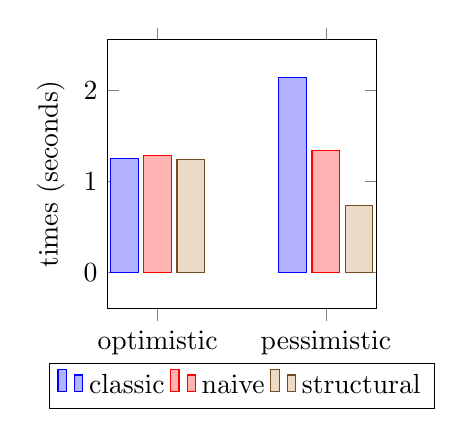
\begin{tikzpicture}
\begin{axis}[
    ybar, ymax = 2, ymin = 0.15,
    enlargelimits=0.3,
    width=5cm, height=5cm,
    legend style={at={(0.5,-0.2)},
      anchor=north,legend columns=-1},
    ylabel={times (seconds)},
    symbolic x coords={optimistic, pessimistic},
    xtick=data
    ]
\addplot coordinates {(optimistic,1.254) (pessimistic,2.142)};
\addplot coordinates {(optimistic,1.282) (pessimistic,1.337)};
\addplot coordinates {(optimistic,1.236) (pessimistic,0.733)};
\legend{classic,naive,structural}
\end{axis}
\end{tikzpicture}
 \captionof{figure}{revers$^o$ forward evaluation \\ for a list with a length of 90}
  \label{fair:plot-reverso}
\end{minipage}%
\begin{minipage}{.5\textwidth}
  \centering
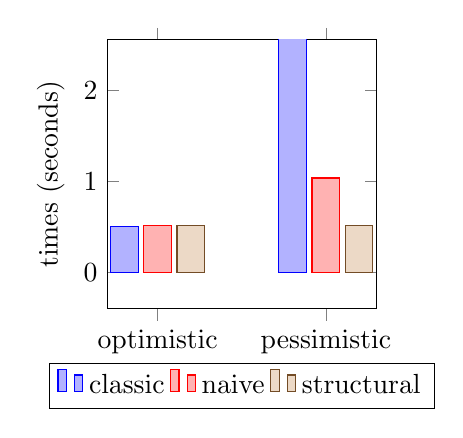
\begin{tikzpicture}
\begin{axis}[
    ybar, ymax = 2, ymin = 0.15,
    enlargelimits=0.3,
    width=5cm, height=5cm,
    legend style={at={(0.5,-0.2)},
      anchor=north,legend columns=-1},
    ylabel={times (seconds)},
    symbolic x coords={optimistic, pessimistic},
    xtick=data
    ]
\addplot coordinates {(optimistic,0.504) (pessimistic,300)};
\addplot coordinates {(optimistic,0.508) (pessimistic,1.035)};
\addplot coordinates {(optimistic,0.513) (pessimistic,0.513)};
\legend{classic,naive,structural}
\end{axis}
\end{tikzpicture}
 \captionof{figure}{sort$^o$ forward evaluation \\ for a list with a length of 5}
\label{fair:plot-sorto}
\end{minipage}
\end{figure*}

\begin{figure*}
\centering
\begin{minipage}{.5\textwidth}
  \centering
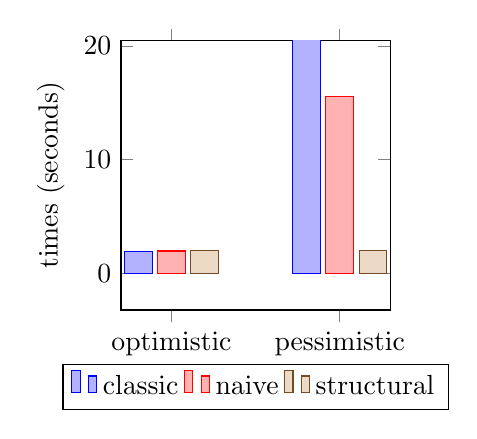
\begin{tikzpicture}
\begin{axis}[
    ybar, ymax = 16, ymin = 1.2,
    enlargelimits=0.3,
    width=5cm, height=5cm,
    legend style={at={(0.5,-0.2)},
      anchor=north,legend columns=-1},
    ylabel={times (seconds)},
    symbolic x coords={optimistic, pessimistic},
    xtick=data
    ]
\addplot coordinates {(optimistic,1.909) (pessimistic,300)};
\addplot coordinates {(optimistic,1.945) (pessimistic,15.516)};
\addplot coordinates {(optimistic,1.980) (pessimistic,1.978)};
\legend{classic,naive,structural}
\end{axis}
\end{tikzpicture}
 \captionof{figure}{``The Tower of Hanoi'' \\ solver evaluation}
\label{fair:plot-hanoi}
\end{minipage}%
\begin{minipage}{.5\textwidth}
  \centering
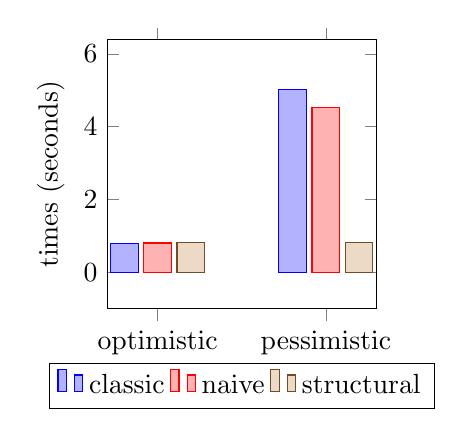
\begin{tikzpicture}
\begin{axis}[
    ybar, ymax = 5, ymin = 0.375,
    enlargelimits=0.3,
    width=5cm, height=5cm,
    legend style={at={(0.5,-0.2)},
      anchor=north,legend columns=-1},
    ylabel={times (seconds)},
    symbolic x coords={optimistic, pessimistic},
    xtick=data
    ]
\addplot coordinates {(optimistic,0.783) (pessimistic,5.019)};
\addplot coordinates {(optimistic,0.801) (pessimistic,4.522)};
\addplot coordinates {(optimistic,0.812) (pessimistic,0.817)};
\legend{classic,naive,structural}
\end{axis}
\end{tikzpicture}
 \captionof{figure}{``Bridge and torch problem'' \\ solver evaluation}
\label{fair:plot-bridge}
\end{minipage}
\end{figure*}

Now we will discuss evaluation. Целью эвалюации является выявления влияния порядка конъюнктов на эффективность трех различных семантик.

Первая семантика с предикатом $pred_{\mbox{\lstinline{true}}}$ близка к классическим реализациям \mk. В дальнейшем будем называть её {\bf left-biased}.

Вторая семантика с предикатом $pred_N$ соответсвует равномерному вычислению всех конъюнктов. Эту семантику будем назвать {\bf naive}.

Третья семантика с предикатом $pred_{\leq_{sr}}$ вычисляет структурно-рекурсивные конъюнкты, пока убывают структурно-рекурсивные аргументы. Её будем называть {\bf structural}.

For evaluation we've chosen two simple programs (list reversing and list sorting) and three more complicated (the ``Hanoi Towers''\footnote{\url{https://en.wikipedia.org/wiki/Tower_of_Hanoi}} solver, the
``Bridge and torch problem''\footnote{\url{https://en.wikipedia.org/wiki/Bridge_and_torch_problem}} solver and ``Water pouring puzzle''\footnote{\url{https://en.wikipedia.org/wiki/Water_pouring_puzzle}} solver).
% Для каждой программы мы сделали две версии. Оптимистичная версия --- это программа, в которой мы вручную подобрали оптимальный порядок конъюнктов и пессиместичная версия --- программа с неоптимальным порядком конъюнктов. В последующих диаграммах и таблице указаны средние значения 10 запусков тестов. Также для наивной равномерной конъюнкции мы подобрали количество разверток вручную. Для равномерной конъюнкции, основанной на структурной рекурсии, N было фиксировано и равно 100.
Each program was written in two versions: ``optimistic'' (with the order of important conjuncts set to provide the best performance) and ``pessimistic'' (with the order of important
conjuncts set to provide the worst performance). Also we evaluated list reversing and list sorting in both directions. In the case of the list reversing, queries \lstinline{(revers$^o$ [1;2;3] q)} and \lstinline{(revers$^o$ q [1;2;3])}\! will give the same answer \lstinline{q = [3;2;1]} but the ``optimistic'' order of conjuncts is different for them. In the case of list sorting, queries \lstinline{(sort$^o$ [1;2;3] q)} and \lstinline{(sort$^o$ q [1;2;3])} will give different answers. The first one gives sorted list \lstinline{q = [1;2;3]}, the second one gives all permutations of list \lstinline{[1;2;3]}\!\!. 

All benchmarks were run ten times, and the average time was taken. For the naive  semantics we cherry-picked the best value of unfolding bound manually. Structural arguments for each relations were detected automatically.

% На изображениях 12-15 представлены результаты апробации в виде столбцовых диаграмм. В оптимистичном случае результаты схожи для всех семантик. В пессиместичном случае время работы напрпавленной конъюнкции резко возрастает, время работы наивной равномерной конъюнкции также ворзрастает, но не так сильно. Равномерная конъюнкция, основанная на структурной рекурсии, демострирует схожую эффективность в сравнении с оптимистичным случаем.
Fig.~\ref{fair:plot-reverso}-\ref{fair:plot-bridge} show the results of evaluation in the form of bar charts. In the optimistic case, the results are similar for all semantics.
In the pessimistic case the evaluation time of the directed conjunction rapidly increases, the evaluation time of the naive fair conjunction also increases, but not so much.
The fair semantics based on structural recursion demonstrates a similar efficiency as in the optimistic case.

\begin{figure*} %[h!]
  \small
  \centering
  \begin{tabular}{ c | c | c | c | c | c | c | c }
    \multirow{2}{*}{relation} & \multirow{2}{*}{size} & 
    \multicolumn{2}{c}{left-biased semantics} &
    \multicolumn{2}{c}{naive semantics} &
    \multicolumn{2}{c}{structural semantics} \\
    \cline{3-8}
    & & optimistic & pessimistic & optimistic & pessimistic & optimistic & pessimistic  \\ 
    \hline
    \multirow{3}{*}{\begin{tabular}{c} forward \\ revers$^o$ \end{tabular}}
                 & 30   & 0.527 & 0.587  & 0.532 & 0.595   & 0.539 & 0.532 \\
                 & 60   & 0.639 & 0.947  & 0.643 & 0.790   & 0.657 & 0.577 \\
                 & 90   & 1.254 & 2.142  & 1.282 & 1.337   & 1.236 & 0.733 \\
    \hline
    \multirow{3}{*}{\begin{tabular}{c} backward \\ revers$^o$ \end{tabular}}
                 & 30   & 0.531 & 0.579  & 0.547 & 0.570  & 0.553 & 0.563 \\
                 & 60   & 0.655 & 0.875  & 0.667 & 0.812  & 0.668 & 0.681 \\
                 & 90   & 1.316 & 1.813  & 1.327 & 1.503  & 1.360 & 1.359 \\
    \hline
    \multirow{5}{*}{\begin{tabular}{c} forward \\ sort$^o$ \end{tabular}}
                 & 3    & 0.467 & 0.503  & 0.474 & 0.481  & 0.472 & 0.479 \\
                 & 4    & 0.484 & 4.679  & 0.485 & 0.493  & 0.490 & 0.488 \\
                 & 5    & 0.504 & $>$300 & 0.508 & 1.035  & 0.513 & 0.513 \\
                 & 6    & 0.526 & $>$300 & 0.237 & 14.369 & 0.544 & 0.547 \\
                 & 30   & 1.915 & $>$300 & 1.936 & $>$300 & 1.983 & 1.987 \\
    \hline
    \multirow{4}{*}{\begin{tabular}{c} backward \\ sort$^o$ \end{tabular}}
                 & 3    & 0.518 &  0.519 & 0.518 & 0.521  & 0.520 & 0.521 \\
                 & 4    & 0.533 &  0.856 & 0.534 & 0.540  & 0.534 & 0.537 \\
                 & 5    & 0.680 & 93.914 & 0.713 & 1.528  & 0.718 & 0.714 \\
                 & 6    & 2.931 & $>$300 & 2.947 & 59.647 & 2.938 & 2.936 \\
    \hline
    hanoi$^o$    & -    & 1.909 & $>$300 & 1.945 & 15.516 & 1.980 & 1.978 \\
    \hline
    bridge$^o$   & -    & 0.783 & 5.019  & 0.801 & 4.522  & 0.812 & 0.817 \\
    \hline
    water$^o$    & -    & 3.513 & $>$300 & 3.518 & $>$300 & 3.538 & 3.771

  \end{tabular}
  \caption{The results of evaluation: running times of benchmarks in seconds}
  \label{fair:evaluation-table}
\end{figure*}

% Более подробно результаты представлены на изображении 16. Можно заметить, что время работы программы sorto в пессиместичном случае очень быстро растет с увеличением длины списка для направленной конъюнкции и наивной равномерной. В случае с равномерной конъюнкцией, основанной на структурной рекурсии, пессиместичный случай растет сопостовимо с оптимистичным.
The results are presented in more detail in Fig.~\ref{fair:evaluation-table}. ``Hanoi Towers'' solver has name \lstinline{hanoi$^o$}, ``Bridge and torch problem'' solver has name \lstinline{bridge$^o$} and ``Water pouring puzzle'' solver has name \lstinline{water$^o$}. We can conclude that forward and backward \lstinline{sort$^o$} runtime in the pessimistic case increases very rapidly with increasing the list length for left-biased and naive fair semantics. In the case of the fair semantics based on structural recursion the running time in pessimistic case increases on a par with that in the optimistic one. Also the solver \lstinline{water$^o$} very slow in the pessimistic case for left-biased and naive fair. However, fair conjunction based on structural recursion pessimistic case is no different from an optimistic case.


% Подводя итог, равномерная конъюнкция, основанная на структурной рекурсии сопоставима по эффективности с направленной конъюнкцией. Более того, это конъюнкция слабо зависит от порядка конъюнктов.
To summarize, the fair semantics based on structural recursion does not introduce any essential overhead in comparison with left-biased semantics in an optimistic case. At the same time it
weakly depends on the order of the conjuncts, and thus demonstrates much better performance in the pessimistic case.

\section{Related works}
\label{sec:related}

Although semantics of pattern matching can be given as a sequence of srutinee's sub expression comparisons (Figure~\ref{fig:matchpatts}) effective compilers don't follow this approach. One can either optimise runtime cost by minimizing amount of checks performed or static cost by minimizing the size of generated code. \emph{Decision trees} are good for the first criteria, because they check every subexpression not more than once. \emph{Backtracking automata} are rather compact but in some cases can perform repeated checks.


Minimizing the size of decision tree is  NP-hard (\cite{macqueen1985}, without proof) and usually various heuristics are applied during compilation, for example: count of nodes, length of the longest path, average length of all paths. The paper~\cite{Ramsey2000} performs experimental evaluation of these heuristics.

The matching compilers for strict languages can work in \emph{direct} or \emph{indirect} styles. The first ones return effective code immediately. In the second style to construct final answer some post processing is required. It can vary from easy simplifications to complicated supercompilation techniques~\cite{Setsoft1996}. The main drawback of indirect style is that size of intermediate data structures can be exponentially large.

For strict languages it is allowed to check sub expressions in any order. For lazy languages pattern matching should evaluate only these sub expressions which are necessary for performing pattern matching, if not careful pattern matching can change termination behavior of the program.  In general lazy languages setup more constraints on pattern matching and because of that allow lesser set of heuristics.

A few approaches for checking sub expressions in lazy langauges has been proposed~\cite{Augustsson1985,Laville1991}. \cite{laville1991} models values in lazy languages using \emph{partial terms}, although this approach doesn't scale to types with infinite constructor sets (like integers). In  the \cite{suarez1993} the similar approach is extended by special treatment of overlapping patterns. Pattern matching has been compiled to decision trees~\cite{maranget1992} and later \cite{maranget1992} into \emph{decision DAGs} that allow in some cases to make code smaller.

TODO: mention 3 papers about strict languages.

\section{Conclusion}
\label{conclusion}

We presented an approach for converting typed functional programs into relations. Relational conversion 
in many cases allows us to avoid tedious recoding of functional specifications into relational form and to 
concentrate on writing relational specifications only when their reconstruction from functions is impossible or 
undesirable. Our implementation works for the subset of OCaml; we evaluated it for a number of interesting 
examples and acquired some new relational solutions.

There is a number of directions for future research. First, a performance evaluation is desirable~--- at
present time we do not know, what slowdown factor is. Another problem is a development of an approach to
prove complete correctness (or refute this claim).


\begin{acks}
  We would like to express our gratitude to the anonymous reviewers for their valuable comments and suggestions.
\end{acks}

\section{Appendix}
\label{appendix}

In this appendix we present a proof of partial semantic correctness of relational conversion, or, to be precise, 
a number of observations, definitions, and claims, which, we believe, are sufficient to reconstruct
the complete proof. 

We remind, that our goal is to prove the following statement:

\begin{theorem} 
\normalfont For arbitrary functional program $p$ of a ground type $t$, arbitrary value $v$, and
arbitrary variable $x$

$$
\begin{array}{c}
p\leadsto^f v \Rightarrow \lstinline|fresh ($x$) ($\sembr{p}^c x$)| \leadsto^r (\theta, \emptyset)\\
\mbox{and}\\
\theta(\mathfrak{s})=v
\end{array}
$$

\noindent where $\mathfrak{s}$ is a semantic variable, associated with
$x$ on the first step of the relational evaluation.
\end{theorem}
  
We first comment on the empty set as the set of negative substitutions. A disequality constraint can
come only from a polymorphic equality, which is applied when both its operands are reduced to
values. In the relational counterpart, being run in a forward direction, this corresponds to the evaluation of disequality constraints for
closed terms only, which, in turn, means, that they will immediately succeed or fail. Both cases
add nothing to the set of negative substitutions, which is initially empty. 

Next, we cannot prove the theorem, using an induction by a derivation length, since in the case of
application, for example, the type of the term in the head position is not ground. This 
obstacle could be lifted, if we could prove the following generalization:

$$
p\leadsto^f f \Rightarrow \sembr{p}^c\leadsto^r\sembr{f}^c
$$ 

\noindent for arbitrary $p$ of any type. This claim, however, turned out to be false~--- a term
\lstinline|C ((fun x.x) A)| can be taken as an example.  

The origin of the problem is that we \emph{functionalize} the constructors, \lstinline|match|, and
equality expressions, and, hence, change the order of reductions in the relational counterpart in 
comparison with the original functional program. Thus, we need to take this change into account.

First, we develop a modified functional semantics, which corresponds better to the reduction
order in the relational case. We call this semantics \emph{deferred}, as it defers the evaluation
of constructors, \lstinline|match|, and equality expressions. This semantics can be acquired in
two steps: first, we consider a reduced version of the original functional semantics, in which
we treat arbitrary constructor, \lstinline|match|, and equality expressions as values. Then, the
deferred semantics is just an iterative application of the reduced version to the arguments 
of these new values (arguments of constructors or equality operator, or scrutinees of \lstinline|match| 
expressions).

Next, we claim, that if a term of some ground type is reduced to some value by the original semantics,
then it as well is reduced to the same value by the deferred one. This claim is based on the following
observations:

\begin{itemize}
\item progress and type preservation properties for both semantics (which can be proven in a standard
way);
\item Church-Rosser property for lambda-calculus;
\item the fact, that the reduced semantics applies a proper subset of rules of the original one.
\end{itemize}

Now, we are going to prove the theorem by a simulation between the deferred semantics for the original program
and the relational one for the relationally converted. Before that, we formulate the number of lemmas and 
definitions.

\begin{lemma}
\label{stack_split}
\normalfont Let us separate all the contexts into two disjoint kinds: 

\begin{itemize}
\item functional

$$
C_f = \Box\;e\mid v\;\Box\mid\lstinline|let $x$ = $\Box$ in $e$|
$$

\item ground

$$
C_g = \lstinline|match $\;\Box\;$ with $\{p_i$->$e_i\}$|\mid C^n(\bar{v},\Box,\bar{e})\mid\Box\lstinline|=e|\mid\lstinline|v=|\Box
$$

Let $\left<{\mathcal S},\,e\right>$ be an arbitrary state in a derivation sequence w.r.t. the deferred
semantics. Then $\mathcal S=C_f^*C_g^*$.
\end{itemize}

In other words, during the evaluation w.r.t. the deferred semantics, the stack of contexts is separated into the two
(possibly empty) segments: all ground contexts reside below all functional. The proof is by the induction on the
length of derivation sequence.
\end{lemma}

\begin{definition}
\normalfont
We as well separate all terms of the source language into the two disjoint kinds:

\begin{itemize}
\item functional

$$
e_1\,e_2\mid \lambda x.e \mid \mu f.\lambda x.e \mid \lstinline|let $x$ = $e_1$ in $e_2$| \mid \lstinline|let rec $f$ = $\lambda x.e_1$ in $e_2$|
$$

\item ground

$$
e_1 = e_2 \mid \lstinline|match $e$ with {$p_i$ -> $e_i$ }| \mid \lstinline|C$^k$ ($e_1\dots e_k$)|
$$

\end{itemize}

\end{definition}

\begin{definition}
\normalfont Augmented conversion of a term w.r.t. to a substitution $\sembr{\bullet}_\theta$ is defined as follows: 

$$
\begin{array}{rcl}
\sembr{p}_\theta&=&\sembr{p}^c\\
\sembr{v}_\theta&=&(\lambda x.x\equiv\mathfrak{s}),\,\mbox{if}\;\;\theta(\mathfrak s)=v
\end{array}
$$

Here $\theta$ is a substitution, $p$~--- arbitrary functional term, $v$~--- arbitrary value of a
ground type in the sense of the original semantics (i.e. the composition of constructors). Note, the
cases in this definition are not disjoint, and in the second case there can be more, than one
variable with the requested property, so augmented conversion defines a set of relational terms.
\end{definition}

\begin{lemma}
\label{substitution}
\normalfont Let $f$, $e$ be two arbitrary terms of the source language, $\theta$~--- arbitrary
substitution. Then

$$
\sembr{f[x\gets e]}_\theta=\sembr{f}_\theta[x\gets\sembr{e}_\theta]
$$

The equality here is understood in a set-theoretic sense. The proof is by structural 
induction.
\end{lemma}

\begin{definition}
\normalfont For arbitrary substitution $\theta$ define a conversion of a functional context  
$\sembr{\bullet}_\theta$ as follows:

$$
\begin{array}{rcl}
\sembr{\Box\,e}_\theta&=&\Box\,\sembr{e}_\theta\\
\sembr{v\,\Box}_\theta&=&\sembr{v}_\theta\,\Box\\
\sembr{\lstinline|let $\;x\; = \;\Box\;$ in $\;e$|}_\theta&=&\lstinline|let $\;x\; = \;\Box\;$ in $\;\sembr{e}_\theta$|
\end{array}
$$

Here $e$ is an arbitrary functional term, $v$~--- abstraction. This conversion is an extension of augmented
conversion for functional contexts, hence the same denotation.
\end{definition}

\begin{definition}
\normalfont For arbitrary semantic variables ${\mathfrak s}_1$, ${\mathfrak s}_2$ and arbitrary substitution $\theta$ 
define a conversion of ground context $\sembr{\bullet}^{{\mathfrak s}_1{\mathfrak s}_2}_\theta$ as follows:

$$ 
\begin{array}{rcl}
\sembr{C^k(v_1, \ldots, v_{i-1}, \Box, e_{i+1}, \ldots, e_k)}^{{\mathfrak s}_1{\mathfrak s}_2}_\theta&=&\Box \; \wedge \\
       & & (\sembr{e_{i+1}}_\theta \; {\mathfrak s}^\prime_{i+1}) \; \wedge \\
       & & \ldots  \\
       & & (\sembr{e_k}_\theta \; {\mathfrak s}^\prime_k) \; \wedge \\
       & & ({\mathfrak s}_2 \equiv\; \uparrow C^k({\mathfrak s}^\prime_1, \ldots, {\mathfrak s}^\prime_{i-1}, {\mathfrak s}_1, {\mathfrak s}^\prime_{i+1}, \ldots, {\mathfrak s}_k)),\,\mbox{if}\;\theta({\mathfrak s}^\prime_j)=v_j,\,j<i
\end{array}
$$

$$
\begin{array}{rcl}
\sembr{\Box = e}^{{\mathfrak s}_1{\mathfrak s}_2}_\theta&=&\Box\, \wedge \\
 & & (\sembr{e}_\theta\; {\mathfrak s}^\prime) \wedge \\
 & & ((({\mathfrak s}_1 \equiv {\mathfrak s}^\prime) \wedge ({\mathfrak s}_2 \equiv \lstinline|^true|))\, \vee \\ 
 & & (({\mathfrak s}_1 \not \equiv {\mathfrak s}^\prime) \wedge ({\mathfrak s}_2 \equiv \lstinline|^false|))) 
\end{array}
$$

$$
\begin{array}{rcl}
\sembr{v = \Box}^{{\mathfrak s}_1{\mathfrak s}_2}_\theta&=&\Box\,\wedge \\
 & & ((({\mathfrak s}^\prime \equiv {\mathfrak s}_1) \wedge ({\mathfrak s}_2 \equiv \lstinline|^true|))\, \vee \\ 
 & & (({\mathfrak s}^\prime \not \equiv {\mathfrak s}_1) \wedge ({\mathfrak s}_2 \equiv \lstinline|^false|))),\,\mbox{if}\;\theta({\mathfrak s})=v 
\end{array}
$$

$$
\begin{array}{rcl}
\sembr{\lstinline|match $\;\Box\;$ with \{$C^{n_i}_i$($y^i_1$, ..., $y^i_{n_i}$) -> $\;e_i$\}|}^{{\mathfrak s}_1{\mathfrak s}_2}_\theta&=&\Box \; \wedge \bigvee_i\\
& &(\lstinline|fresh ($s^i_1 \ldots s^i_{n_i}$)| \\
& &\qquad({\mathfrak s}_1 \equiv \;\uparrow C_i^{n_i}(s^i_1, \ldots, s^i_{n_i})) \\
& &\qquad(\lambda y^i_1. \ldots \lambda  y^i_{n_i}. \sembr{e_i}_\theta) \; (\equiv s^i_1) \ldots (\equiv s^i_{n_i})\;{\mathfrak s}_2)
\end{array}
$$

Here we assume ${\mathfrak s}^\prime$ and ${\mathfrak s}^\prime_i$ to be arbitrary semantic variables, $v_i$~--- arbitrary values w.r.t. the original 
functional semantics, $e_i$~--- arbitrary terms of the source language. We also claim, that $\theta$ is
undefined for all mentioned semantic variables, unless the opposite is specified explicitly.

\end{definition}

\begin{definition}
\normalfont For arbitrary substitution $\theta$, arbitrary semantic variable ${\mathfrak s}_m$ and a functional 
term $e$ define a conversion of a stack $\sembr{\bullet}^{e,{\mathfrak s}_m}_\theta$ as follows:

$$
\def\arraystretch{1.5}
\sembr{f_n\dots f_1g_m\dots g_1}^{e,{\mathfrak s}_m}_\theta=\left\{
\begin{array}{lcl}
\sembr{g_m}^{{\mathfrak s}_m{\mathfrak s}_{m-1}}_\theta\dots\sembr{g_1}^{{\mathfrak s}_1{\mathfrak s}_0}_\theta&,&n=0\;\;\mbox{and $e$~--- ground}\\
\sembr{f_n}_\theta\dots\sembr{f_1}_\theta(\Box\,{\mathfrak s}_m)\sembr{g_m}^{{\mathfrak s}_m{\mathfrak s}_{m-1}}_\theta\dots\sembr{g_1}^{{\mathfrak s}_1{\mathfrak s}_0}_\theta&,&\mbox{otherwise}
\end{array}
\right.
$$

Here ${\mathfrak s}_0\dots {\mathfrak s}_{m-1}$ designate arbitrary distinct semantic variables.
\end{definition}

\begin{definition}
\normalfont For arbitrary substitution $\theta$ and arbitrary semantic variable ${\mathfrak s}_m$ define a simulation
conversion $\sembr{\bullet}^{{\mathfrak s}_m}_\theta$ of the source language term as follows:

$$
\begin{array}{rcl}
\sembr{e_1 = e_2}^{{\mathfrak s}_m}_\theta&=& (\sembr{e_1}_\theta\; {\mathfrak s}^\prime_1) \wedge \\
                           & & (\sembr{e_2}_\theta\; {\mathfrak s}^\prime_2) \wedge \\
                           & & ((({\mathfrak s}^\prime_1 \equiv {\mathfrak s}^\prime_2) \wedge ({\mathfrak s}_m \equiv \lstinline|^true|))\, \vee \\ 
                           & & (({\mathfrak s}^\prime_1 \not \equiv {\mathfrak s}^\prime_2) \wedge ({\mathfrak s}_m \equiv \lstinline|^false|)))
\end{array}
$$

$$
\begin{array}{rcl}
\sembr{v = e}^{{\mathfrak s}_m}_\theta&=& (\sembr{e}_\theta\; {\mathfrak s}^\prime_2) \wedge \\
                        & & ((({\mathfrak s}^\prime_1 \equiv {\mathfrak s}^\prime_2) \wedge ({\mathfrak s}_m \equiv \lstinline|^true|))\, \vee \\ 
                        & & (({\mathfrak s}^\prime_1 \not \equiv {\mathfrak s}^\prime_2) \wedge ({\mathfrak s}_m \equiv \lstinline|^false|))),\,\mbox{if}\;\theta({\mathfrak s}^\prime_1)=v
\end{array}
$$

$$
\begin{array}{rcl}
\sembr{v_1 = v_2}^{{\mathfrak s}_m}_\theta&=& ((({\mathfrak s}^\prime_1 \equiv {\mathfrak s}^\prime_2) \wedge ({\mathfrak s}_m \equiv \lstinline|^true|))\, \vee \\ 
                           & & (({\mathfrak s}^\prime_1 \not \equiv {\mathfrak s}^\prime_2) \wedge ({\mathfrak s}_m \equiv \lstinline|^false|))),\,\mbox{if}\;\theta({\mathfrak s}^\prime_j)=v_j
\end{array}
$$

$$ 
\begin{array}{rcl}
\sembr{C^k(v_1, \ldots, v_{i-1}, e_i, \ldots, e_k)}^{{\mathfrak s}_m}_\theta&=&(\sembr{e_i}_\theta \; {\mathfrak s}^\prime_i) \; \wedge \\
       & & \ldots  \\
       & & (\sembr{e_k}_\theta \; {\mathfrak s}^\prime_k) \; \wedge \\
       & & ({\mathfrak s}_m \equiv\; \uparrow C^k({\mathfrak s}^\prime_1, \ldots, {\mathfrak s}^\prime_k)),\,\mbox{if}\;\theta({\mathfrak s}^\prime_j)=v_j,\,j<i
\end{array}
$$

$$ 
\sembr{C^k(v_1, \ldots, v_k)}^{{\mathfrak s}_m}_\theta = ({\mathfrak s}_m \equiv\; \uparrow C^k({\mathfrak s}^\prime_1, \ldots, {\mathfrak s}^\prime_k)),\,\mbox{if}\;\theta({\mathfrak s}^\prime_j)=v_j
$$

$$ 
\sembr{C^k(v_1, \ldots, v_k)}^{{\mathfrak s}_m}_\theta = ({\mathfrak s}_m \equiv\; {\mathfrak s}^\prime),\;\mbox{if}\;\theta({\mathfrak s}^\prime)=C^k(v_1, \ldots, v_k)
$$

$$
\begin{array}{rcl}
\sembr{\lstinline|match $\;e\;$ with \{$C^{n_i}_i$($y^i_1$, ..., $y^i_{n_i}$) -> $\;e_i$\}|}^{{\mathfrak s}_m}_\theta&=&\sembr{e}_\theta\;{\mathfrak s}^\prime\;\wedge\;\bigvee_i\\
& &(\lstinline|fresh ($s^i_1 \ldots s^i_{n_i}$)| \\
& &\qquad({\mathfrak s}^\prime \equiv \;\uparrow C_i^{n_i}(s^i_1, \ldots, s^i_{n_i})) \\
& &\qquad(\lambda y^i_1. \ldots \lambda  y^i_{n_i}. \sembr{e_i}_\theta) \; (\equiv s^i_1) \ldots (\equiv s^i_{n_i})\;{\mathfrak s}_m)
\end{array}
$$

$$
\begin{array}{rcl}
\sembr{\lstinline|match $\;v\;$ with \{$C^{n_i}_i$($y^i_1$, ..., $y^i_{n_i}$) -> $\;e_i$\}|}^{{\mathfrak s}_m}_\theta&=&\bigvee_i\\
& &(\lstinline|fresh ($s^i_1 \ldots s^i_{n_i}$)| \\
& &\qquad({\mathfrak s}^\prime \equiv \;\uparrow C_i^{n_i}(s^i_1, \ldots, s^i_{n_i})) \\
& &\qquad(\lambda y^i_1. \ldots \lambda  y^i_{n_i}. \sembr{e_i}_\theta) \; (\equiv s^i_1) \ldots (\equiv s^i_{n_i})\;{\mathfrak s}_m),\,\mbox{if}\;\theta({\mathfrak s}^\prime)=v
\end{array}
$$

Here all ${\mathfrak s}^\prime$ and ${\mathfrak s}^\prime_i$ designate arbitrary semantic variables, $e$~--- arbitrary term, $v$~--- arbitrary value w.r.t. the
original semantics. We also claim, that $\theta$ is undefined for all mentioned semantic variables, unless the opposite is specified explicitly.
\end{definition}

\begin{definition}
\normalfont Let 
\begin{itemize}
\item \mbox{$\left<\mathcal S,\,e\right>$}~--- a state w.r.t. the deferred semantics;
\item \mbox{$\left<\Sigma, \hat{\mathcal S}, \hat{e}, (\theta, \emptyset)\right>$}~--- a state w.r.t. the
relational semantics.
\end{itemize} 

We say, that these states are connected, if there exists a semantic variable $q_m$, such, that:\vspace{1mm}

\begin{enumerate}
\item \mbox{$\hat{\mathcal S}\in\sembr{\mathcal S}^{e,{\mathfrak s}_m}_\theta$}\vspace{1mm}
\item \mbox{$\hat{e}\in\left\{
                          \begin{array}{lcl}
                            \sembr{e}^{{\mathfrak s}_m}_\theta&,&e\mbox{~--- ground and }\mathcal S\mbox{ does not contain functional contexts}\\[1mm]
                            \sembr{e}_\theta&,&\mbox{otherwise}
                          \end{array}
                       \right.
            $} 
\item $\Sigma$ contains all semantic variables from $\hat{e}$, $\hat{\mathcal S}$, and $\theta$.
\end{enumerate}

\end{definition}

\begin{lemma}
\label{constructor}
\normalfont Let $v=\lstinline|C$^k$($v_1$,...,$v_k$)|$ be a value. Then
for arbitrary $\Sigma$, $\mathcal S$, $\theta$, $\hat{v}\in \sembr{v}_\theta$, and 
semantic variable ${\mathfrak s}$, such, that ${\mathfrak s}\not\in dom(\theta)$ either

$$
\left<\Sigma,\,\mathcal S, (\hat{v}\,{\mathfrak s}),\, (\theta,\,\emptyset)\right>\leadsto^*\left<\Sigma^\prime,\,\mathcal S,\,{\mathfrak s}\equiv\lstinline|C$^k$(${\mathfrak s}^\prime_1$,...,${\mathfrak s}^\prime_k$)|,\,(\theta^\prime,\,\emptyset)\right>\;\mbox{and}\;\theta^\prime({\mathfrak s}^\prime_i)=v_i
$$

or

$$
\left<\Sigma,\,\mathcal S, (\hat{v}\,{\mathfrak s}),\, (\theta,\,\emptyset)\right>\leadsto\left<\Sigma,\,\mathcal S,\,{\mathfrak s}\equiv {\mathfrak s}^\prime,\,(\theta,\,\emptyset)\right>\;\mbox{and}\;\theta({\mathfrak s}^\prime)=v
$$
 
The proof is by induction on the height of $v$.
\end{lemma}

\begin{lemma}
\label{evaluation_lemma}
\normalfont Let $s=\left<\mathcal S=g_m\dots g_1,\,e\right>$ be a state w.r.t. the deferred semantics, 
$g_i$~--- ground contexts, $e$~--- expression of a ground type, $\theta$~--- some substitution,
${\mathfrak s}_m$~--- some semantic variable, \mbox{$\hat{\mathcal{S}}\in\sembr{\mathcal S}^{e,\,{\mathfrak s}_m}_\theta$}, 
\mbox{$\hat{e} \in \sembr{e}_\theta$}. Then there is a sequence of steps w.r.t. the relational
semantics, such, that

$$
\left<\Sigma, \hat{\mathcal S}, (\hat{e} \, {\mathfrak s}_m), (\theta,\,\emptyset) \right>\leadsto^*\hat{s}
$$

\noindent and $s$ and $\hat{s}$ are connected. Here we assume $\Sigma$ to contain all semantic variables from
$\hat{\mathcal S}$ and $\theta$. The proof is by case analysis on $e$, using Lemma~\ref{constructor}.
\end{lemma}

\begin{lemma} 
\label{connection}
\normalfont Let \mbox{$s_1 \to s_2$}~--- a single evaluation step w.r.t. the deferred semantics,
$\hat{s_1}$~--- a state of the relational semantics, such, that $s_1$ and $\hat{s_1}$ are connected. Then
there exists a sequence of steps in the relational semantics \mbox{$\hat{s_1}\leadsto^*\hat{s_2}$}, such, 
that $s_2$ and $\hat{s_2}$ are connected. The proof is by case analysis and definition of connection
relation, using Lemmas~\ref{substitution},~\ref{constructor},~\ref{evaluation_lemma}. 
\end{lemma}

\begin{lemma}
\label{prefix}
\normalfont Let $s_0=\left<\emptyset,\,\epsilon,\,\lstinline|fresh ($x$) $(\sembr{e}^c\;x)$|,\,\iota\right>$ be an
initial state of evaluation w.r.t. the relational semantics. Then there is a sequence of steps
\mbox{$s_0\leadsto^*\hat{s}$}, such, that \mbox{$\left<\epsilon,\,e\right>$} (an initial state of
evaluation of $e$ w.r.t. the deferred semantics) and $\hat{s}$ are connected. Immediately follows from
Lemma~\ref{evaluation_lemma}.
\end{lemma}

Now we can prove the partial correctness theorem. Let us have a term $e$ of a ground type in the source language, which
reduces to a value $v=\lstinline|C$^k$($v_1$,...,$v_k$)|$ w.r.t. the original call-by-value semantics. Then it reduces to the same value w.r.t. the
deferred semantics: 

$$
\left<\epsilon,\,e\right>\to^*\left<\epsilon,\,v\right>
$$

By Lemma~\ref{prefix} 

$$
\left<\emptyset,\,\epsilon,\lstinline|fresh ($x$) $(\sembr{e}^c\;x)$|,\iota\right>\leadsto^*\hat{s}
$$

\noindent where \mbox{$\left<\epsilon,\,e\right>$} and $\hat{s}$ are connected. By Lemma~\ref{connection}, there is
a state $\hat{s^\prime}$ w.r.t. the relational semantics, such, that

$$
\hat{s}\leadsto^*\hat{s^\prime}
$$

\noindent and \mbox{$\left<\epsilon,\,v\right>$} and $\hat{s^\prime}$ are connected. By the definition of
the connection relation, $\hat{s^\prime}$ has one of the following forms:

$$
\left<\Sigma,\,\epsilon,\,{\mathfrak s}_0\equiv\lstinline|C$^k$(${\mathfrak s}^\prime_1$,...,${\mathfrak s}^\prime_k$)|,\,(\theta,\,\emptyset)\right>,\,\theta({\mathfrak s}^\prime_i)=v_i
$$

\noindent or

$$
\left<\Sigma,\,\epsilon,\,{\mathfrak s}_0\equiv {\mathfrak s}^\prime,\,(\theta,\,\emptyset)\right>,\,\theta({\mathfrak s}^\prime)=v
$$

\noindent where ${\mathfrak s}_0$ is the first semantic variable, added to $\Sigma$, and \mbox{${\mathfrak s}_0\not\in dom(\theta)$}. In
both cases, we can make the one last step in the relational semantics, which completes the proof. 


\bibliographystyle{ACM-Reference-Format}
\bibliography{fair-conj}

\end{document}
\endinput
%%
%% End of file `sample-sigplan.tex'.
